\documentclass[10pt,fleqn]{article} % Default font size and left-justified equations
\usepackage[%
    pdftitle={Informatique : Numpy},
    pdfauthor={Xavier Pessoles}]{hyperref}
    
%%%%%%%%%%%%%%%%%%%%%%%%%%%%%%%%%%%%%%%%%
% Original author:
% Mathias Legrand (legrand.mathias@gmail.com) with modifications by:
% Vel (vel@latextemplates.com)
% License:
% CC BY-NC-SA 3.0 (http://creativecommons.org\newtheorem{rappelT}{Rappel}[section]/licenses/by-nc-sa/3.0/)
%%%%%%%%%%%%%%%%%%%%%%%%%%%%%%%%%%%%%%%%%

%----------------------------------------------------------------------------------------
%	VARIOUS REQUIRED PACKAGES AND CONFIGURATIONS
%----------------------------------------------------------------------------------------

\usepackage[top=2.5cm,bottom=2cm,left=2cm,right=2cm,headsep=40pt,a4paper]{geometry} % Page margins

\usepackage{graphicx} % Required for including pictures
\graphicspath{{images/}} % Specifies the directory where pictures are stored
\usepackage{float}

\usepackage{lipsum} % Inserts dummy text

\usepackage{tikz} % Required for drawing custom shapes

\usepackage[french]{babel} % English language/hyphenation
\frenchbsetup{StandardLists=true} % Pour éviter la collision babel enumitem pour les listes

\usepackage{enumitem} % Customize lists
\setlist{nolistsep} % Reduce spacing between bullet points and numbered lists

\usepackage{booktabs} % Required for nicer horizontal rules in tables

\usepackage{colortbl} % Couleur dans les tableaux

\usepackage{xcolor} % Required for specifying colors by name
%\definecolor{ocre}{RGB}{243,102,25} % Define the orange color used for highlighting throughout the book
\definecolor{ocre}{RGB}{49,133,156} % Couleur ''bleue''
\definecolor{violetf}{RGB}{112,48,160} % Couleur ''violet''
\usepackage{enumitem}
\usepackage{pifont} % Pour les dinglist
\usepackage{multicol}
\usepackage{array} % Centrage vertical dans les tableaux

%----------------------------------------------------------------------------------------
%	FONTS
%----------------------------------------------------------------------------------------

\usepackage{avant} % Use the Avantgarde font for headings
%\usepackage{times} % Use the Times font for headings
%\usepackage{mathptmx} % Use the Adobe Times Roman as the default text font together with math symbols from the Sym­bol, Chancery and Com­puter Modern fonts
\usepackage[adobe-utopia]{mathdesign}
\usepackage{microtype} % Slightly tweak font spacing for aesthetics
\usepackage[utf8]{inputenc} % Required for including letters with accents
\usepackage[T1]{fontenc} % Use 8-bit encoding that has 256 glyphs

%----------------------------------------------------------------------------------------
%	BIBLIOGRAPHY AND INDEX
%----------------------------------------------------------------------------------------

\usepackage[style=alphabetic,citestyle=numeric,sorting=nyt,sortcites=true,autopunct=true,babel=hyphen,hyperref=true,abbreviate=false,backref=true,backend=biber]{biblatex}
\addbibresource{bibliography.bib} % BibTeX bibliography file
\defbibheading{bibempty}{}

\usepackage{calc} % For simpler calculation - used for spacing the index letter headings correctly
\usepackage{makeidx} % Required to make an index
\makeindex % Tells LaTeX to create the files required for indexing

%----------------------------------------------------------------------------------------
%	MAIN TABLE OF CONTENTS
%----------------------------------------------------------------------------------------

\usepackage{titletoc} % Required for manipulating the table of contents

\setcounter{tocdepth}{2}     % Dans la table des matieres
\setcounter{secnumdepth}{2}

\contentsmargin{0cm} % Removes the default margin

% Part text styling
\titlecontents{part}[0cm]
{\addvspace{20pt}\centering\large\bfseries}
{}
{}
{}

% Chapter text styling
\titlecontents{chapter}[1.25cm] % Indentation
{\addvspace{12pt}\large\sffamily\bfseries} % Spacing and font options for chapters
{\color{ocre!60}\contentslabel[\Large\thecontentslabel]{1.25cm}\color{ocre}} % Chapter number
{\color{ocre}}  
{\color{ocre!60}\normalsize\;\titlerule*[.5pc]{.}\;\thecontentspage} % Page number

% Section text styling
\titlecontents{section}[1.25cm] % Indentation
{\addvspace{3pt}\sffamily\bfseries} % Spacing and font options for sections
{\color{ocre!60}\contentslabel[\thecontentslabel]{1.25cm} \color{ocre}} % Section number
{\color{ocre}}
{\hfill\color{ocre!60}\thecontentspage} % Page number
[]

% Subsection text styling
\titlecontents{subsection}[1.25cm] % Indentation
{\addvspace{1pt}\sffamily\small} % Spacing and font options for subsections
{\contentslabel[\thecontentslabel]{1.25cm}} % Subsection number
{}
{\ \titlerule*[.5pc]{.}\;\thecontentspage} % Page number
[]


% Subsection text styling
\titlecontents{subsubsection}[1.25cm] % Indentation
{\addvspace{1pt}\sffamily\small} % Spacing and font options for subsections
{\contentslabel[\thecontentslabel]{1.25cm}} % Subsection number
{}
{\ \titlerule*[.5pc]{.}\;\thecontentspage} % Page number
[]

% List of figures
\titlecontents{figure}[0em]
{\addvspace{-5pt}\sffamily}
{\thecontentslabel\hspace*{1em}}
{}
{\ \titlerule*[.5pc]{.}\;\thecontentspage}
[]

% List of tables
\titlecontents{table}[0em]
{\addvspace{-5pt}\sffamily}
{\thecontentslabel\hspace*{1em}}
{}
{\ \titlerule*[.5pc]{.}\;\thecontentspage}
[]

%----------------------------------------------------------------------------------------
%	MINI TABLE OF CONTENTS IN PART HEADS
%----------------------------------------------------------------------------------------

% Chapter text styling
\titlecontents{lchapter}[0em] % Indenting
{\addvspace{15pt}\large\sffamily\bfseries} % Spacing and font options for chapters
{\color{ocre}\contentslabel[\Large\thecontentslabel]{1.25cm}\color{ocre}} % Chapter number
{}  
{\color{ocre}\normalsize\sffamily\bfseries\;\titlerule*[.5pc]{.}\;\thecontentspage} % Page number

% Section text styling
\titlecontents{lsection}[0em] % Indenting
{\sffamily\small} % Spacing and font options for sections
{\contentslabel[\thecontentslabel]{1.25cm}} % Section number
{}
{}

% Subsection text styling
\titlecontents{lsubsection}[.5em] % Indentation
{\normalfont\footnotesize\sffamily} % Font settings
{}
{}
{}

%----------------------------------------------------------------------------------------
%	PAGE HEADERS
%----------------------------------------------------------------------------------------

\usepackage{fancyhdr} % Required for header and footer configuration



\pagestyle{fancy}
 \renewcommand{\headrulewidth}{0pt}
 \fancyhead{}
 \fancyhead[L]{%
 \noindent\begin{minipage}[c]{2.6cm}%
 
\includegraphics[width=2cm]{png/logo_lycee.png}%
 \end{minipage}}

\fancyhead[C]{\rule{8cm}{.5pt}}

 \fancyhead[R]{%
 \noindent\begin{minipage}[c]{3cm}
 \begin{flushright}
 \footnotesize{\textit{\textsf{\xxtete}}}%
 \end{flushright}
 \end{minipage}
}


\fancyfoot[C]{\rule{12cm}{.5pt}}
\renewcommand{\footrulewidth}{0.2pt}
\fancyfoot[C]{\footnotesize{\bfseries \thepage}}
\fancyfoot[L]{ 
\begin{minipage}[c]{.2\linewidth}
\noindent\footnotesize{{\xxauteur}}
\end{minipage}}


\fancyfoot[R]{\footnotesize{\xxpied}
\ifthenelse{\isodd{\value{page}}}{
\begin{tikzpicture}[overlay]
\node[shape=rectangle, 
      rounded corners = .25 cm,
	  draw= ocre,
	  line width=2pt, 
	  fill = ocre!10,
	  minimum width  = 2.5cm,
	  minimum height = 3cm,] at (\xxposongletx,\xxposonglety) {};
\node at (\xxposonglettext,\xxposonglety) {\rotatebox{90}{\textbf{\large\color{ocre}{\xxonglet}}}};
%{};
\end{tikzpicture}}{}
}
%
%
%
% Removes the header from odd empty pages at the end of chapters
\makeatletter
\renewcommand{\cleardoublepage}{
\clearpage\ifodd\c@page\else
\hbox{}
\vspace*{\fill}
\thispagestyle{empty}
\newpage
\fi}

\fancypagestyle{plain}{%
\fancyhf{} % vide l’en-tête et le pied~de~page.
%\fancyfoot[C]{\bfseries \thepage} % numéro de la page en cours en gras
% et centré en pied~de~page.
\fancyfoot[R]{\footnotesize{\xxpied}}
\fancyfoot[C]{\rule{12cm}{.5pt}}
\renewcommand{\footrulewidth}{0.2pt}
\fancyfoot[C]{\footnotesize{\bfseries \thepage}}
\fancyfoot[L]{ 
\begin{minipage}[c]{.2\linewidth}
\noindent\footnotesize{{\xxauteur}}
\end{minipage}}}



%----------------------------------------------------------------------------------------
%	THEOREM STYLES
%----------------------------------------------------------------------------------------

% Conflit avec la police adobe
%\usepackage{amsmath,amsfonts,amssymb,amsthm} % For math equations, theorems, symbols, etc
\usepackage{amsmath,amsthm}

\newcommand{\intoo}[2]{\mathopen{]}#1\,;#2\mathclose{[}}
\newcommand{\ud}{\mathop{\mathrm{{}d}}\mathopen{}}
\newcommand{\intff}[2]{\mathopen{[}#1\,;#2\mathclose{]}}
%\newtheorem{notation}{Notation}[chapter]
\newtheorem{notation}{Notation}[section]

% Boxed/framed environments
\newtheoremstyle{ocrenumbox}% % Theorem style name
{0pt}% Space above
{0pt}% Space below
{\normalfont}% % Body font
{}% Indent amount
{\small\bf\sffamily\color{ocre}}% % Theorem head font
{\;}% Punctuation after theorem head
{0.25em}% Space after theorem head
{\small\sffamily\color{ocre}\thmname{#1}\nobreakspace\thmnumber%{\@ifnotempty{#1}{}\@upn{#2}}% Theorem text (e.g. Theorem 2.1)
\thmnote{\nobreakspace\the\thm@notefont\sffamily\bfseries\color{black}---\nobreakspace#3.}} % Optional theorem note
\renewcommand{\qedsymbol}{$\blacksquare$}% Optional qed square


% Boite pour les corriges
\newtheoremstyle{correctionbox}% % Theorem style name
{0pt}% Space above
{0pt}% Space below
{\normalfont}% % Body font
{}% Indent amount
{\small\bf\sffamily\color{violet}}% % Theorem head font
{\;}% Punctuation after theorem head
{0.25em}% Space after theorem head
{\small\sffamily\color{ocre}\thmname{#1}\nobreakspace\thmnumber%{\@ifnotempty{#1}{}\@upn{#2}}% Theorem text (e.g. Theorem 2.1)
\thmnote{\nobreakspace\the\thm@notefont\sffamily\bfseries\color{black}---\nobreakspace#3.}} % Optional theorem note
\renewcommand{\qedsymbol}{$\blacksquare$}% Optional qed square



\newtheoremstyle{blacknumex}% Theorem style name
{5pt}% Space above
{5pt}% Space below
{\normalfont}% Body font
{} % Indent amount
{\small\bf\sffamily}% Theorem head font
{\;}% Punctuation after theorem head
{0.25em}% Space after theorem head
{\small\sffamily{\tiny\ensuremath{\blacksquare}}\nobreakspace\thmname{#1}\nobreakspace\thmnumber%{\@ifnotempty{#1}{}\@upn{#2}}% Theorem text (e.g. Theorem 2.1)
\thmnote{\nobreakspace\the\thm@notefont\sffamily\bfseries---\nobreakspace#3.}}% Optional theorem note

\newtheoremstyle{blacknumbox} % Theorem style name
{0pt}% Space above
{0pt}% Space below
{\normalfont}% Body font
{}% Indent amount
{\small\bf\sffamily}% Theorem head font
{\;}% Punctuation after theorem head
{0.25em}% Space after theorem head
{\small\sffamily\thmname{#1}\nobreakspace 
\thmnote{\nobreakspace\the\thm@notefont\sffamily\bfseries---\nobreakspace#3.}}% Optional theorem note

% Non-boxed/non-framed environments
\newtheoremstyle{ocrenum}% % Theorem style name
{5pt}% Space above
{5pt}% Space below
{\normalfont}% % Body font
{}% Indent amount
{\small\bf\sffamily\color{ocre}}% % Theorem head font
{\;}% Punctuation after theorem head
{0.25em}% Space after theorem head
{\small\sffamily\color{ocre}\thmname{#1}\nobreakspace%\thmnumber{\@ifnotempty{#1}{}\@upn{#2}}% Theorem text (e.g. Theorem 2.1)
\thmnote{\nobreakspace\the\thm@notefont\sffamily\bfseries\color{black}---\nobreakspace#3.}} % Optional theorem note
\renewcommand{\qedsymbol}{$\blacksquare$}% Optional qed square
\makeatother

% Environnement pour les titres de parties
\newtheoremstyle{partiebox} 
{0pt}% Space above
{0pt}% Space below
{\normalfont}% Body font
{}% Indent amount
{\small\bf\sffamily}% Theorem head font
{\;}% Punctuation after theorem head
{0.25em}% Space after theorem head




% Defines the theorem text style for each type of theorem to one of the three styles above
\newcounter{dummy} 
\numberwithin{dummy}{section}
\theoremstyle{ocrenumbox}
%\newtheorem{theoremeT}[dummy]{Théorème}
\newtheorem{theoremeT}[dummy]{Théorème}
\newtheorem{resultatT}[dummy]{Résultat}
\newtheorem{savoirT}[dummy]{Savoir}
\newtheorem{methodeT}[dummy]{Méthode}
\newtheorem{objectifT}[dummy]{Objectif}
%\newtheorem{problem}{Problem}[chapter]
\newtheorem{problem}{Problem}[section]
%\newtheorem{exerciseT}{Exercise}[chapter]
\newtheorem{exerciseT}{Exercice}[section]

\theoremstyle{blacknumex}
%\newtheorem{exampleT}{Example}[chapter]
\newtheorem{exempleT}{Exemple}[section]
\newtheorem{termT}{Terminal\\}[section]
\newtheorem{pyT}{Python\\}[section]
\newtheorem{sciT}{Scilab\\}[section]
\newtheorem{pseudoT}{Pseudo Code\\}[section]
\newtheorem{sqlT}{SQL\\}[section]

\theoremstyle{blacknumbox}
%\newtheorem{vocabulary}{Vocabulary}[chapter]
\newtheorem{vocabulary}{Vocabulaire}[section]
%\newtheorem{definitionT}{Definition}[section]
\newtheorem{definitionT}{Définition}[section]
\newtheorem{rappelT}{Rappel}[section]
\newtheorem{demoT}{Démonstration}[section]
\newtheorem{corollaryT}[dummy]{Corollaire}
\newtheorem{hypoT}{Hypothèse(s)}

\theoremstyle{ocrenum}
\newtheorem{proposition}[dummy]{Proposition}

\theoremstyle{partiebox}
\newtheorem{titrepartieT}[]{}
\newtheorem{titrechapitreT}[]{}

\theoremstyle{correctionbox}
\newtheorem{correctionT}[dummy]{\color{violet}{Correction}}

%----------------------------------------------------------------------------------------
%	DEFINITION OF COLORED BOXES
%----------------------------------------------------------------------------------------

\RequirePackage[framemethod=tikz]{mdframed} % Required for creating the theorem, definition, exercise and corollary boxes

% Theorem box
\newmdenv[skipabove=7pt,
skipbelow=7pt,
backgroundcolor=ocre!10,
linecolor=ocre,
innerleftmargin=5pt,
innerrightmargin=5pt,
innertopmargin=5pt,
leftmargin=0cm,
rightmargin=0cm,
innerbottommargin=5pt]{tBox}


% Correction
\newmdenv[skipabove=7pt,
skipbelow=7pt,
backgroundcolor=violet!10,
linecolor=violet,
innerleftmargin=5pt,
innerrightmargin=5pt,
innertopmargin=5pt,
leftmargin=0cm,
rightmargin=0cm,
innerbottommargin=5pt]{coBox}


% Exercise box	  
\newmdenv[skipabove=7pt,
skipbelow=7pt,
rightline=false,
leftline=true,
topline=false,
bottomline=false,
backgroundcolor=ocre!10,
linecolor=ocre,
innerleftmargin=5pt,
innerrightmargin=5pt,
innertopmargin=5pt,
innerbottommargin=5pt,
leftmargin=0cm,
rightmargin=0cm,
linewidth=4pt]{eBox}	

% Definition box
\newmdenv[skipabove=7pt,
skipbelow=7pt,
rightline=false,
leftline=true,
topline=false,
bottomline=false,
backgroundcolor=ocre!10,
linecolor=ocre,
innerleftmargin=5pt,
innerrightmargin=5pt,
innertopmargin=1pt,
leftmargin=0cm,
rightmargin=0cm,
linewidth=4pt,
innerbottommargin=0pt]{dBox}	

% Demonstration box
\newmdenv[skipabove=7pt,
skipbelow=7pt,
rightline=false,
leftline=true,
topline=false,
bottomline=false,
%backgroundcolor=ocre!10,
linecolor=ocre,
innerleftmargin=5pt,
innerrightmargin=5pt,
innertopmargin=0pt,
leftmargin=0cm,
rightmargin=0cm,
linewidth=4pt,
innerbottommargin=0pt]{demoBox}	

% Corollary box
\newmdenv[skipabove=7pt,
skipbelow=7pt,
rightline=false,
leftline=true,
topline=false,
bottomline=false,
linecolor=gray,
backgroundcolor=black!5,
innerleftmargin=5pt,
innerrightmargin=5pt,
innertopmargin=5pt,
leftmargin=0cm,
rightmargin=0cm,
linewidth=4pt,
innerbottommargin=5pt]{cBox}


% Hypothèses
\newmdenv[skipabove=7pt,
skipbelow=7pt,
rightline=false,
leftline=true,
topline=false,
bottomline=false,
linecolor=gray,
backgroundcolor=black!5,
innerleftmargin=5pt,
innerrightmargin=5pt,
innertopmargin=5pt,
leftmargin=0cm,
rightmargin=0cm,
linewidth=4pt,
innerbottommargin=5pt]{hyBox}


% Boite pour le titre de la partie (pBox)
\newmdenv[skipabove=7pt,
skipbelow=7pt,
rightline=true,
leftline=false,
topline=false,
bottomline=false,
linecolor=ocre,
backgroundcolor=none,
innerleftmargin=5pt,
innerrightmargin=5pt,
innertopmargin=5pt,
leftmargin=0cm,
rightmargin=0cm,
linewidth=4pt,
innerbottommargin=5pt]{pBox}

% Boite pour le titre du chapitre (chBox)
\newmdenv[skipabove=7pt,
skipbelow=7pt,
rightline=false,
leftline=true,
topline=false,
bottomline=false,
linecolor=ocre,
%backgroundcolor=black!5,
innerleftmargin=5pt,
innerrightmargin=5pt,
innertopmargin=5pt,
leftmargin=0cm,
rightmargin=0cm,
linewidth=4pt,
innerbottommargin=5pt]{chBox}


% Boite pour les exemples
\newmdenv[skipabove=7pt,
skipbelow=7pt,
rightline=false,
leftline=true,
topline=false,
bottomline=false,
linecolor=gray,
backgroundcolor=white,
innerleftmargin=5pt,
innerrightmargin=5pt,
innertopmargin=5pt,
leftmargin=0cm,
rightmargin=0cm,
linewidth=4pt,
innerbottommargin=5pt]{exBox}

% Boite pour le terminal
\newmdenv[skipabove=7pt,
skipbelow=7pt,
rightline=false,
leftline=true,
topline=false,
bottomline=false,
linecolor=gray,
backgroundcolor=white,
innerleftmargin=5pt,
innerrightmargin=5pt,
innertopmargin=5pt,
leftmargin=0cm,
rightmargin=0cm,
linewidth=4pt,
innerbottommargin=5pt]{termBox}


% Boite pour Python
\newmdenv[skipabove=7pt,
skipbelow=7pt,
rightline=false,
leftline=true,
topline=false,
bottomline=false,
linecolor=gray,
backgroundcolor=white,
innerleftmargin=5pt,
innerrightmargin=5pt,
innertopmargin=5pt,
leftmargin=0cm,
rightmargin=0cm,
linewidth=4pt,
innerbottommargin=5pt]{pyBox}

% Boite pour scilab
\newmdenv[skipabove=7pt,
skipbelow=7pt,
rightline=false,
leftline=true,
topline=false,
bottomline=false,
linecolor=gray,
backgroundcolor=white,
innerleftmargin=5pt,
innerrightmargin=5pt,
innertopmargin=5pt,
leftmargin=0cm,
rightmargin=0cm,
linewidth=4pt,
innerbottommargin=5pt]{sciBox}


% Boite pour pseudo
\newmdenv[skipabove=7pt,
skipbelow=7pt,
rightline=false,
leftline=true,
topline=false,
bottomline=false,
linecolor=gray,
backgroundcolor=white,
innerleftmargin=5pt,
innerrightmargin=5pt,
innertopmargin=5pt,
leftmargin=0cm,
rightmargin=0cm,
linewidth=4pt,
innerbottommargin=5pt]{pseudoBox}

% Boite pour pseudo
\newmdenv[skipabove=7pt,
skipbelow=7pt,
rightline=false,
leftline=true,
topline=false,
bottomline=false,
linecolor=gray,
backgroundcolor=white,
innerleftmargin=5pt,
innerrightmargin=5pt,
innertopmargin=5pt,
leftmargin=0cm,
rightmargin=0cm,
linewidth=4pt,
innerbottommargin=5pt]{sqlBox}


% Creates an environment for each type of theorem and assigns it a theorem text style from the "Theorem Styles" section above and a colored box from above
\newenvironment{theorem}{\begin{tBox}\begin{theoremeT}}{\end{theoremeT}\end{tBox}}
\newenvironment{resultat}{\begin{tBox}\begin{resultatT}}{\end{resultatT}\end{tBox}}
\newenvironment{methode}{\begin{tBox}\begin{methodeT}}{\end{methodeT}\end{tBox}}
\newenvironment{savoir}{\begin{tBox}\begin{savoirT}}{\end{savoirT}\end{tBox}}
\newenvironment{obj}{\begin{tBox}\begin{objectifT}}{\end{objectifT}\end{tBox}}
\newenvironment{corrige}{\begin{coBox}\begin{correctionT}}{\end{correctionT}\end{coBox}}
\newenvironment{exercise}{\begin{eBox}\begin{exerciseT}}{\hfill{\color{ocre}\tiny\ensuremath{\blacksquare}}\end{exerciseT}\end{eBox}}				  
\newenvironment{exercice}{\begin{eBox}\begin{exerciseT}}{\hfill{\color{ocre}\tiny\ensuremath{\blacksquare}}\end{exerciseT}\end{eBox}}				  

\newenvironment{definition}{\begin{dBox}\begin{definitionT}}{\end{definitionT}\end{dBox}}	
\newenvironment{defi}{\begin{dBox}\begin{definitionT}}{\end{definitionT}\end{dBox}}	
\newenvironment{demo}{\begin{demoBox}\begin{demoT}}{\end{demoT}\end{demoBox}}	
\newenvironment{rappel}{\begin{dBox}\begin{rappelT}}{\end{rappelT}\end{dBox}}	
%\newenvironment{exemple}{\begin{exempleT}}{\hfill{\tiny\ensuremath{\blacksquare}}\end{exempleT}}		
\newenvironment{corollary}{\begin{cBox}\begin{corollaryT}}{\end{corollaryT}\end{cBox}}
\newenvironment{hypo}{\begin{hyBox}\begin{hypoT}}{\end{hypoT}\end{hyBox}}	\newenvironment{exemple}{\begin{exBox}\begin{exempleT}}{\hfill{\tiny\ensuremath{\blacksquare}}\end{exempleT}\end{exBox}}	
\newenvironment{titrepartie}{\begin{pBox}\begin{titrepartieT}}{\end{titrepartieT}\end{pBox}}	
\newenvironment{titrechapitre}{\begin{chBox}\begin{titrechapitreT}}{\end{titrechapitreT}\end{chBox}}	

\newenvironment{term}{ \begin{termBox}\begin{termT}}{\end{termT}\end{termBox}}
\newenvironment{py}{ \begin{pyBox}\begin{pyT}}{\end{pyT}\end{pyBox}}
\newenvironment{sci}{ \begin{sciBox}\begin{sciT}}{\end{sciT}\end{sciBox}}
\newenvironment{pseudo}{ \begin{pseudoBox}\begin{pseudoT}}{\end{pseudoT}\end{pseudoBox}}
\newenvironment{envsql}{ \begin{sqlBox}\begin{sqlT}}{\end{sqlT}\end{sqlBox}}


%----------------------------------------------------------------------------------------
%	REMARK ENVIRONMENT
%----------------------------------------------------------------------------------------

\newenvironment{remark}{\par\vspace{10pt}\small % Vertical white space above the remark and smaller font size
\begin{list}{}{
\leftmargin=35pt % Indentation on the left
\rightmargin=25pt}\item\ignorespaces % Indentation on the right
\makebox[-2.5pt]{\begin{tikzpicture}[overlay]
\node[draw=ocre!60,line width=1pt,circle,fill=ocre!25,font=\sffamily\bfseries,inner sep=2pt,outer sep=0pt] at (-15pt,0pt){\textcolor{ocre}{R}};\end{tikzpicture}} % Orange R in a circle
\advance\baselineskip -1pt}{\end{list}\vskip5pt} % Tighter line spacing and white space after remark

\newenvironment{rem}{\par\vspace{10pt}\small % Vertical white space above the remark and smaller font size
\begin{list}{}{
\leftmargin=35pt % Indentation on the left
\rightmargin=25pt}\item\ignorespaces % Indentation on the right
\makebox[-2.5pt]{\begin{tikzpicture}[overlay]
\node[draw=ocre!60,line width=1pt,circle,fill=ocre!25,font=\sffamily\bfseries,inner sep=2pt,outer sep=0pt] at (-15pt,0pt){\textcolor{ocre}{R}};\end{tikzpicture}} % Orange R in a circle
\advance\baselineskip -1pt}{\end{list}\vskip5pt} % Tighter line spacing and white space after remark


\newenvironment{warn}{\par\vspace{10pt}\small % Vertical white space above the remark and smaller font size
\begin{list}{}{
\leftmargin=35pt % Indentation on the left
\rightmargin=25pt}\item\ignorespaces % Indentation on the right
\makebox[-2.5pt]{\begin{tikzpicture}[overlay]
\node[draw=red!60,line width=1pt,circle,fill=red!25,font=\sffamily\bfseries,inner sep=2pt,outer sep=0pt] at (-15pt,0pt){\textcolor{black}{!}};\end{tikzpicture}} % Point d'exclamation dans un cercle
\advance\baselineskip -1pt}{\end{list}\vskip5pt} % Tighter line spacing and white space after remark


%----------------------------------------------------------------------------------------
%	SECTION NUMBERING IN THE MARGIN
%----------------------------------------------------------------------------------------
\setcounter{secnumdepth}{3}
\setcounter{tocdepth}{2}



\makeatletter
\renewcommand{\@seccntformat}[1]{\llap{\textcolor{ocre}{\csname the#1\endcsname}\hspace{1em}}}                    
\renewcommand{\section}{\@startsection{section}{1}{\z@}
{-4ex \@plus -1ex \@minus -.4ex}
{1ex \@plus.2ex }
{\normalfont\large\sffamily\bfseries}}
\renewcommand{\subsection}{\@startsection {subsection}{2}{\z@}
{-3ex \@plus -0.1ex \@minus -.4ex}
{0.5ex \@plus.2ex }
{\normalfont\sffamily\bfseries}}
\renewcommand{\subsubsection}{\@startsection {subsubsection}{3}{\z@}
{-2ex \@plus -0.1ex \@minus -.2ex}
{.2ex \@plus.2ex }
{\normalfont\small\sffamily\bfseries}}                        
\renewcommand\paragraph{\@startsection{paragraph}{4}{\z@}
{-2ex \@plus-.2ex \@minus .2ex}
{.1ex}
{\normalfont\small\sffamily\bfseries}}

%----------------------------------------------------------------------------------------
%	PART HEADINGS
%----------------------------------------------------------------------------------------


%----------------------------------------------------------------------------------------
%	CHAPTER HEADINGS
%----------------------------------------------------------------------------------------

% \newcommand{\thechapterimage}{}%
% \newcommand{\chapterimage}[1]{\renewcommand{\thechapterimage}{#1}}%
% \def\@makechapterhead#1{%
% {\parindent \z@ \raggedright \normalfont
% \ifnum \c@secnumdepth >\m@ne
% \if@mainmatter
% \begin{tikzpicture}[remember picture,overlay]
% \node at (current page.north west)
% {\begin{tikzpicture}[remember picture,overlay]
% \node[anchor=north west,inner sep=0pt] at (0,0) {\includegraphics[width=\paperwidth]{\thechapterimage}};
% \draw[anchor=west] (\Gm@lmargin,-9cm) node [line width=2pt,rounded corners=15pt,draw=ocre,fill=white,fill opacity=0.5,inner sep=15pt]{\strut\makebox[22cm]{}};
% \draw[anchor=west] (\Gm@lmargin+.3cm,-9cm) node {\huge\sffamily\bfseries\color{black}\thechapter. #1\strut};
% \end{tikzpicture}};
% \end{tikzpicture}
% \else
% \begin{tikzpicture}[remember picture,overlay]
% \node at (current page.north west)
% {\begin{tikzpicture}[remember picture,overlay]
% \node[anchor=north west,inner sep=0pt] at (0,0) {\includegraphics[width=\paperwidth]{\thechapterimage}};
% \draw[anchor=west] (\Gm@lmargin,-9cm) node [line width=2pt,rounded corners=15pt,draw=ocre,fill=white,fill opacity=0.5,inner sep=15pt]{\strut\makebox[22cm]{}};
% \draw[anchor=west] (\Gm@lmargin+.3cm,-9cm) node {\huge\sffamily\bfseries\color{black}#1\strut};
% \end{tikzpicture}};
% \end{tikzpicture}
% \fi\fi\par\vspace*{270\p@}}}

%-------------------------------------------

\def\@makeschapterhead#1{%
\begin{tikzpicture}[remember picture,overlay]
\node at (current page.north west)
{\begin{tikzpicture}[remember picture,overlay]
\node[anchor=north west,inner sep=0pt] at (0,0) {\includegraphics[width=\paperwidth]{\thechapterimage}};
\draw[anchor=west] (\Gm@lmargin,-9cm) node [line width=2pt,rounded corners=15pt,draw=ocre,fill=white,fill opacity=0.5,inner sep=15pt]{\strut\makebox[22cm]{}};
\draw[anchor=west] (\Gm@lmargin+.3cm,-9cm) node {\huge\sffamily\bfseries\color{black}#1\strut};
\end{tikzpicture}};
\end{tikzpicture}
\par\vspace*{270\p@}}
\makeatother

%----------------------------------------------------------------------------------------
%	HYPERLINKS IN THE DOCUMENTS
%----------------------------------------------------------------------------------------


\hypersetup{hidelinks,backref=true,pagebackref=true,hyperindex=true,colorlinks=false,breaklinks=true,urlcolor= ocre,bookmarks=true,bookmarksopen=false,pdftitle={Title},pdfauthor={Author}}
\usepackage{bookmark}
\bookmarksetup{
open,
numbered,
addtohook={%
\ifnum\bookmarkget{level}=0 % chapter
\bookmarksetup{bold}%
\fi
\ifnum\bookmarkget{level}=-1 % part
\bookmarksetup{color=ocre,bold}%
\fi
}
}

%----------------------------------------------------------------------------------------
%	
%----------------------------------------------------------------------------------------

\newcommand{\thechapterimage}{}%
\newcommand{\chapterimage}[1]{\renewcommand{\thechapterimage}{#1}}%
\def\@makechapterhead#1{%
{\parindent \z@ \raggedright \normalfont
\begin{tikzpicture}[remember picture,overlay]
\node at (current page.north west)
{\begin{tikzpicture}[remember picture,overlay]
\node[anchor=north west,inner sep=0pt] at (0,0) {\includegraphics[width=\paperwidth]{\thechapterimage}};
%\draw[anchor=west] (\Gm@lmargin,-9cm) node [line width=2pt,rounded corners=15pt,draw=ocre,fill=white,fill opacity=0.5,inner sep=15pt]{\strut\makebox[22cm]{}};
%\draw[anchor=west] (\Gm@lmargin+.3cm,-9cm) node {\huge\sffamily\bfseries\color{black}\thechapter. #1\strut};
\end{tikzpicture}};
\end{tikzpicture}
\par\vspace*{270\p@}
}}


\newcounter{exo}


\makeatletter             
\renewcommand{\subparagraph}{\@startsection{exo}{5}{\z@}%
                                    {-2ex \@plus-.2ex \@minus .2ex}%
                                    {0ex}%               
{\normalfont\bfseries Question \hspace{.7cm} }}
\makeatother
\renewcommand{\thesubparagraph}{\arabic{subparagraph}} 
\makeatletter



%\makeatletter             
%\renewcommand{\subparagraph}{\@startsection{subparagraph}{5}{\z@}%
%                                    {-2ex \@plus-.2ex \@minus .2ex}%
%                                    {0ex}%               
%{\normalfont\bfseries Question \hspace{.7cm} }}
%\makeatother
%\renewcommand{\thesubparagraph}{\arabic{subparagraph}} 
%\makeatletter


%%%% Environnement pour inclure du code
\usepackage{textcomp}
\usepackage[french]{algorithm2e}
\usepackage{listings}
\lstloadlanguages{R}   % pour regler les pb d accent utf8 dans les codes
\lstset{language=R} % pour regler les pb d accent utf8 dans les codes
\renewcommand{\lstlistlistingname}{Listings}
\renewcommand{\lstlistingname}{Listing}

\SetKwBlock{Fonction}{Début Fonction}{Fin Fonction}
\SetKwComment{Comment}{start}{end}

\definecolor{Bleu}{rgb}{0.1,0.1,1.0}
\definecolor{Noir}{rgb}{0,0,0}
\definecolor{Grau}{rgb}{0.5,0.5,0.5}
\definecolor{DunkelGrau}{rgb}{0.15,0.15,0.15}
\definecolor{Hellbraun}{rgb}{0.5,0.25,0.0}
\definecolor{Magenta}{rgb}{1.0,0.0,1.0}
\definecolor{Gris}{gray}{0.5}
\definecolor{Vert}{rgb}{0,0.5,0}
\definecolor{SourceHintergrund}{rgb}{1,1.0,0.95}


\lstnewenvironment{python}[1][]{
\lstset{
%escapeinside={\%*}{*)},
inputencoding=utf8,   % pour regler les pb d accent utf8 dans les codes
extendedchars=true,   % pour regler les pb d accent utf8 dans les codes
language=python,
basicstyle=\ttfamily\footnotesize, 	
stringstyle=\color{red}, 
showstringspaces=false, 
alsoletter={1234567890},
otherkeywords={\ , \}, \{},
keywordstyle=\color{blue},
emph={access,and,break,class,continue,def,del,elif ,else,
except,exec,finally,for,from,global,if,import,in,i s,
lambda,not,or,pass,print,raise,return,try,while},
emphstyle=\color{black}\bfseries,
emph={[2]True, False, None, self},
emphstyle=[2]\color{black},
emph={[3]from, import, as},
emphstyle=[3]\color{blue},
upquote=true,
columns=flexible, % pour empecher d'avoir un espacement mono
morecomment=[s]{"""}{"""},
commentstyle=\color{Hellbraun}\slshape, 
%emph={[4]1, 2, 3, 4, 5, 6, 7, 8, 9, 0},
emphstyle=[4]\color{blue},
literate=*{:}{{\textcolor{blue}:}}{1}
{=}{{\textcolor{blue}=}}{1}
{-}{{\textcolor{blue}-}}{1}
{+}{{\textcolor{blue}+}}{1}
{*}{{\textcolor{blue}*}}{1}
{!}{{\textcolor{blue}!}}{1}
{(}{{\textcolor{blue}(}}{1}
{)}{{\textcolor{blue})}}{1}
{[}{{\textcolor{blue}[}}{1}
{]}{{\textcolor{blue}]}}{1}
{<}{{\textcolor{blue}<}}{1}
{>}{{\textcolor{blue}>}}{1}
{COMPLETER}{{\textcolor{red}COMPLETER}}{1},
literate=%
            {é}{{\'{e}}}1
            {è}{{\`{e}}}1
            {ê}{{\^{e}}}1
            {ë}{{\¨{e}}}1
            {û}{{\^{u}}}1
            {ù}{{\`{u}}}1
            {â}{{\^{a}}}1
            {à}{{\`{a}}}1
            {î}{{\^{i}}}1
            {ç}{{\c{c}}}1
            {Ç}{{\c{C}}}1
            {É}{{\'{E}}}1
            {Ê}{{\^{E}}}1
            {À}{{\`{A}}}1
            {Â}{{\^{A}}}1
            {Î}{{\^{I}}}1, % pour regler les pb d accent utf8 dans les codes
%framexleftmargin=1mm, framextopmargin=1mm, frame=shadowbox, rulesepcolor=\color{blue},#1
%backgroundcolor=\color{SourceHintergrund}, 
%framexleftmargin=1mm, framexrightmargin=1mm, framextopmargin=1mm, frame=single, framerule=1pt, rulecolor=\color{black},#1
}}{}



\lstnewenvironment{scilab}[1][]{
\lstset{
language=scilab,
basicstyle=\sffamily\footnotesize, 	
stringstyle=\color{red}, 
showstringspaces=false, 
alsoletter={1234567890},
otherkeywords={\ , \}, \{},
keywordstyle=\color{blue},
emph={access,and,break,class,continue,def,del,elif ,else,
except,exec,finally,for,from,global,if,import,in,i s,
lambda,not,or,pass,print,raise,return,try,while,Debut},
emphstyle=\color{black}\bfseries,
emph={[2]True, False, None, self},
emphstyle=[2]\color{black},
emph={[3]from, import, as},
emphstyle=[3]\color{blue},
upquote=true,
columns=flexible, % pour empecher d'avoir un espacement mono
morecomment=[s]{"""}{"""},
commentstyle=\color{Hellbraun}\slshape, 
%emph={[4]1, 2, 3, 4, 5, 6, 7, 8, 9, 0},
emphstyle=[4]\color{blue},
literate=*{:}{{\textcolor{blue}:}}{1}
{=}{{\textcolor{blue}=}}{1}
{-}{{\textcolor{blue}-}}{1}
{+}{{\textcolor{blue}+}}{1}
{*}{{\textcolor{blue}*}}{1}
{!}{{\textcolor{blue}!}}{1}
{(}{{\textcolor{blue}(}}{1}
{)}{{\textcolor{blue})}}{1}
{[}{{\textcolor{blue}[}}{1}
{]}{{\textcolor{blue}]}}{1}
{<}{{\textcolor{blue}<}}{1}
{>}{{\textcolor{blue}>}}{1},
%framexleftmargin=1mm, framextopmargin=1mm, frame=shadowbox, rulesepcolor=\color{blue},#1
%backgroundcolor=\color{SourceHintergrund}, 
%framexleftmargin=1mm, framexrightmargin=1mm, framextopmargin=1mm, frame=single, framerule=1pt, rulecolor=\color{black},#1
}}{}


\lstdefinestyle{stylepython}{%
escapeinside={\%*}{*)},
inputencoding=utf8,   % pour regler les pb d accent utf8 dans les codes
extendedchars=true,   % pour regler les pb d accent utf8 dans les codes
language=python,
basicstyle=\sffamily\footnotesize, 	
stringstyle=\color{red}, 
showstringspaces=false, 
alsoletter={1234567890},
otherkeywords={\ , \}, \{},
keywordstyle=\color{blue},
emph={access,and,break,class,continue,def,del,elif ,else,
except,exec,finally,for,from,global,if,import,in,i s,
lambda,not,or,pass,print,raise,return,try,while},
emphstyle=\color{black}\bfseries,
emph={[2]True, False, None, self},
emphstyle=[2]\color{green},
emph={[3]from, import, as},
emphstyle=[3]\color{blue},
upquote=true,
columns=flexible, % pour empecher d'avoir un espacement mono
morecomment=[s]{"""}{"""},
commentstyle=\color{Hellbraun}\slshape, 
%emph={[4]1, 2, 3, 4, 5, 6, 7, 8, 9, 0},
emphstyle=[4]\color{blue},
literate=*{:}{{\textcolor{blue}:}}{1}
{=}{{\textcolor{blue}=}}{1}
{-}{{\textcolor{blue}-}}{1}
{+}{{\textcolor{blue}+}}{1}
{*}{{\textcolor{blue}*}}{1}
{!}{{\textcolor{blue}!}}{1}
{(}{{\textcolor{blue}(}}{1}
{)}{{\textcolor{blue})}}{1}
{[}{{\textcolor{blue}[}}{1}
{]}{{\textcolor{blue}]}}{1}
{<}{{\textcolor{blue}<}}{1}
{>}{{\textcolor{blue}>}}{1}
{COMPLETER}{{\textcolor{red}COMPLETER}}{1},
literate=%
            {é}{{\'{e}}}1
            {è}{{\`{e}}}1
            {ê}{{\^{e}}}1
            {ë}{{\¨{e}}}1
            {û}{{\^{u}}}1
            {ù}{{\`{u}}}1
            {â}{{\^{a}}}1
            {à}{{\`{a}}}1
            {î}{{\^{i}}}1
            {ç}{{\c{c}}}1
            {Ç}{{\c{C}}}1
            {É}{{\'{E}}}1
            {Ê}{{\^{E}}}1
            {À}{{\`{A}}}1
            {Â}{{\^{A}}}1
            {Î}{{\^{I}}}1,
%numbers=left,                    % where to put the line-numbers; possible values are (none, left, right)
%numbersep=5pt,                   % how far the line-numbers are from the code
%numberstyle=\tiny\color{mygray}, % the style that is used for the line-numbers
}



\lstnewenvironment{termi}[1][]{
\lstset{
language=scilab,
basicstyle=\sffamily\footnotesize, 	
stringstyle=\color{red}, 
showstringspaces=false, 
alsoletter={1234567890},
otherkeywords={\ , \}, \{},
keywordstyle=\color{blue},
emph={access,and,break,class,continue,def,del,elif ,else,
except,exec,finally,for,from,global,if,import,in,i s,
lambda,not,or,pass,print,raise,return,try,while,Debut},
emphstyle=\color{black}\bfseries,
emph={[2]True, False, None, self},
emphstyle=[2]\color{green},
emph={[3]from, import, as},
emphstyle=[3]\color{blue},
upquote=true,
columns=flexible, % pour empecher d'avoir un espacement mono
morecomment=[s]{"""}{"""},
commentstyle=\color{Hellbraun}\slshape, 
%emph={[4]1, 2, 3, 4, 5, 6, 7, 8, 9, 0},
emphstyle=[4]\color{blue},
literate=*{:}{{\textcolor{blue}:}}{1}
{=}{{\textcolor{blue}=}}{1}
{-}{{\textcolor{blue}-}}{1}
{+}{{\textcolor{blue}+}}{1}
{*}{{\textcolor{blue}*}}{1}
{!}{{\textcolor{blue}!}}{1}
{(}{{\textcolor{blue}(}}{1}
{)}{{\textcolor{blue})}}{1}
{[}{{\textcolor{blue}[}}{1}
{]}{{\textcolor{blue}]}}{1}
{<}{{\textcolor{blue}<}}{1}
{>}{{\textcolor{blue}>}}{1},
%framexleftmargin=1mm, framextopmargin=1mm, frame=shadowbox, rulesepcolor=\color{blue},#1
%backgroundcolor=\color{SourceHintergrund}, 
%framexleftmargin=1mm, framexrightmargin=1mm, framextopmargin=1mm, frame=single, framerule=1pt, rulecolor=\color{black},#1
}}{}


\lstnewenvironment{sql}[1][]{
\lstset{
%escapeinside={\%*}{*)},
%inputencoding=utf8,   % pour regler les pb d accent utf8 dans les codes
%extendedchars=true,   % pour regler les pb d accent utf8 dans les codes
language=sql,
basicstyle=\sffamily\footnotesize, 	
stringstyle=\color{red}, 
showstringspaces=false, 
alsoletter={1234567890},
otherkeywords={\ , \}, \{},
keywordstyle=\color{blue},
emph={access,and,break,class,continue,def,del,elif ,else,
except,exec,finally,for,from,global,if,import,in,i s,
lambda,not,or,pass,print,raise,return,try,while},
emphstyle=\color{black}\bfseries,
emph={[2]True, False, None, self},
emphstyle=[2]\color{black},
emph={[3]from, import, as},
emphstyle=[3]\color{blue},
upquote=true,
columns=flexible, % pour empecher d'avoir un espacement mono
morecomment=[s]{"""}{"""},
commentstyle=\color{Hellbraun}\slshape, 
%emph={[4]1, 2, 3, 4, 5, 6, 7, 8, 9, 0},
emphstyle=[4]\color{blue},
literate=*{:}{{\textcolor{blue}:}}{1}
{=}{{\textcolor{blue}=}}{1}
{-}{{\textcolor{blue}-}}{1}
{+}{{\textcolor{blue}+}}{1}
{*}{{\textcolor{blue}*}}{1}
{!}{{\textcolor{blue}!}}{1}
{(}{{\textcolor{blue}(}}{1}
{)}{{\textcolor{blue})}}{1}
{[}{{\textcolor{blue}[}}{1}
{]}{{\textcolor{blue}]}}{1}
{<}{{\textcolor{blue}<}}{1}
{>}{{\textcolor{blue}>}}{1}
{COMPLETER}{{\textcolor{red}COMPLETER}}{1},
literate=%
            {é}{{\'{e}}}1
            {è}{{\`{e}}}1
            {ê}{{\^{e}}}1
            {ë}{{\¨{e}}}1
            {û}{{\^{u}}}1
            {ù}{{\`{u}}}1
            {â}{{\^{a}}}1
            {à}{{\`{a}}}1
            {î}{{\^{i}}}1
            {ç}{{\c{c}}}1
            {Ç}{{\c{C}}}1
            {É}{{\'{E}}}1
            {Ê}{{\^{E}}}1
            {À}{{\`{A}}}1
            {Â}{{\^{A}}}1
            {Î}{{\^{I}}}1, % pour regler les pb d accent utf8 dans les codes
%framexleftmargin=1mm, framextopmargin=1mm, frame=shadowbox, rulesepcolor=\color{blue},#1
%backgroundcolor=\color{SourceHintergrund}, 
%framexleftmargin=1mm, framexrightmargin=1mm, framextopmargin=1mm, frame=single, framerule=1pt, rulecolor=\color{black},#1
}}{}


% Définition des booleéns
\newif\iffiche
\newif\ifprof
\newif\iftd
\newif\ifcours

%%%%%%%%%%%%
% Définition des vecteurs 
%%%%%%%%%%%%
 \newcommand{\vect}[1]{\overrightarrow{#1}}
\newcommand{\axe}[2]{\left(#1,\vect{#2}\right)}

\newcommand{\rep}[1]{\mathcal{R}_{#1}}
\newcommand{\vx}[1]{\vect{x_{#1}}}
\newcommand{\vy}[1]{\vect{y_{#1}}}
\newcommand{\vz}[1]{\vect{z_{#1}}}

%%%%%%%%%%%%
% Définition des torseurs 
%%%%%%%%%%%%

 \newcommand{\torseur}[1]{%
\left\{{#1}\right\}
}

\newcommand{\torseurcin}[3]{%
\left\{\mathcal{#1} \left(#2/#3 \right) \right\}
}

\newcommand{\torseurstat}[3]{%
\left\{\mathcal{#1} \left(#2\rightarrow #3 \right) \right\}
}

 \newcommand{\torseurc}[8]{%
%\left\{#1 \right\}=
\left\{
{#1}
\right\}
 = 
\left\{%
\begin{array}{cc}%
{#2} & {#5}\\%
{#3} & {#6}\\%
{#4} & {#7}\\%
\end{array}%
\right\}_{#8}%
}

 \newcommand{\torseurcol}[7]{
\left\{%
\begin{array}{cc}%
{#1} & {#4}\\%
{#2} & {#5}\\%
{#3} & {#6}\\%
\end{array}%
\right\}_{#7}%
}

 \newcommand{\torseurl}[3]{%
%\left\{\mathcal{#1}\right\}_{#2}=%
\left\{%
\begin{array}{l}%
{#1} \\%
{#2} %
\end{array}%
\right\}_{#3}%
}

 \newcommand{\vectv}[3]{%
\vect{V\left( {#1} \in {#2}/{#3}\right)}
}


\newcommand{\vectf}[2]{%
\vect{R\left( {#1} \rightarrow {#2}\right)}
}

\newcommand{\vectm}[3]{%
\vect{\mathcal{M}\left( {#1}, {#2} \rightarrow {#3}\right)}
}


 \newcommand{\vectg}[3]{%
\vect{\Gamma \left( {#1} \in {#2}/{#3}\right)}
}

 \newcommand{\vecto}[2]{%
\vect{\Omega\left( {#1}/{#2}\right)}
}
% }$$\left\{\mathcal{#1} \right\}_{#2} =%
% \left\{%
% \begin{array}{c}%
%  #3 \\%
%  #4 %
% \end{array}%
% \right\}_{#5}}

\newcommand{\llbr}{\ensuremath{\llbracket}}
\newcommand{\rrbr}{\ensuremath{\rrbracket}}

\usepackage{multicol}
\fichetrue
%\fichefalse

\proftrue
\proffalse

\tdtrue
%\tdfalse

%\courstrue
\coursfalse
\usepackage{siunitx}
% -------------------------------------
% Déclaration des titres
% -------------------------------------

\def\discipline{Informatique}
\def\xxtete{Informatique}
\def\classe{PSI$\star$}
\def\xxnumpartie{}%Partie 5}
\def\xxpartie{Algorithmique \& Programmation (Suite)}

\def\xxnumchapitre{Chapitre 4}
\def\xxchapitre{\hspace{.12cm} Résolution numérique des équations différentielles}

\def\xxtitreexo{Transfert thermique dans un mur}
\def\xxsourceexo{}%\hspace{.2cm} Informatique pour tous en CPGE -- \textit{Wack \& al.}}

\def\xxposongletx{2}
\def\xxposonglettext{1.45}
\def\xxposonglety{13}%10

\def\xxonglet{Ch. 4}%Part. 5 -- Ch. 4}

\def\xxactivite{504}
\def\xxauteur{\textsl{G. Haberer -- X. Pessoles}}

\def\xxcompetences{%
\textsl{%
\textbf{Savoirs et compétences :}
\begin{itemize}[label=\ding{112},font=\color{ocre}] 
\item Problème dynamique à une dimension, linéaire ou non, conduisant à la résolution approchée
d’une équation différentielle ordinaire par la méthode d’Euler (ici, il y aura plusieurs dimensions...)
\item Savoir utiliser une bibliothèque de calcul scientifique. %Alg -- C17 : tris d’un tableau à une dimension de valeurs numériques (tri par insertion, tri %rapide, tri fusion).
\end{itemize}
}}

\def\xxfigures{}%
\includegraphics[width=.75\textwidth]{images/logo}}%figues de la page de garde

\def\xxpied{%
%Partie 5 -- Algorithmique et Programmation\\
Ch 4 : Résolution numérique des équations différentielles -- \xxactivite%
}



\setcounter{secnumdepth}{5}
%---------------------------------------------------------------------------

\begin{document}
\def\columnseprulecolor{\color{ocre}}
\setlength{\columnseprule}{0.4pt} 

%\chapterimage{png/Fond_Cin}
\pagestyle{empty}


%%%%%%%% PAGE DE GARDE COURS
\ifcours
\begin{tikzpicture}[remember picture,overlay]
\node at (current page.north west)
{\begin{tikzpicture}[remember picture,overlay]
\node[anchor=north west,inner sep=0pt] at (0,0) {\includegraphics[width=\paperwidth]{\thechapterimage}};
\draw[anchor=west] (-2cm,-8cm) node [line width=2pt,rounded corners=15pt,draw=ocre,fill=white,fill opacity=0.6,inner sep=40pt]{\strut\makebox[22cm]{}};
\draw[anchor=west] (1cm,-8cm) node {\huge\sffamily\bfseries\color{black} %
\begin{minipage}{1cm}
\rotatebox{90}{\LARGE\sffamily\textsc{\color{ocre}\textbf{\xxnumpartie}}}
\end{minipage} \hfill
\begin{minipage}[c]{14cm}
\begin{titrepartie}
\begin{flushright}
\renewcommand{\baselinestretch}{1.1} 
\Large\sffamily\textsc{\textbf{\xxpartie}}
\renewcommand{\baselinestretch}{1} 
\end{flushright}
\end{titrepartie}
\end{minipage} \hfill
\begin{minipage}[c]{3.5cm}
{\large\sffamily\textsc{\textbf{\color{ocre} \discipline}}}
\end{minipage} 
 };
\end{tikzpicture}};
\end{tikzpicture}


\begin{tikzpicture}[overlay]
\node[shape=rectangle, 
      rounded corners = .25 cm,
	  draw= ocre,
	  line width=2pt, 
	  fill = ocre!10,
	  minimum width  = 2.cm,
	  minimum height = 2.5cm,] at (18cm,-4.7cm) {};
\node at (17.7cm,-4.65) {\rotatebox{90}{\textbf{\Large\color{ocre}{\classe}}}};
%{};
\end{tikzpicture}

\vspace{3.5cm}

\begin{tikzpicture}[remember picture,overlay]
\draw[anchor=west] (-2cm,-6cm) node {\huge\sffamily\bfseries\color{black} %
\begin{minipage}{2cm}
\begin{center}
\LARGE\sffamily\textsc{\color{ocre}\textbf{\xxactivite}}
\end{center}
\end{minipage} \hfill
\begin{minipage}[c]{15cm}
\begin{titrechapitre}
\renewcommand{\baselinestretch}{1.1} 
\Large\sffamily\textsc{\textbf{\xxnumchapitre}}

\Large\sffamily\textsc{\textbf{\xxchapitre}}
\vspace{.5cm}

\renewcommand{\baselinestretch}{1} 
\normalsize\normalfont
\xxcompetences
\end{titrechapitre}
\end{minipage}  };
\end{tikzpicture}
\vfill

\begin{flushright}
\begin{minipage}[c]{.3\linewidth}
\begin{center}
\xxfigures
\end{center}
\end{minipage}\hfill
\begin{minipage}[c]{.6\linewidth}
\startcontents
\printcontents{}{1}{}
\end{minipage}
\end{flushright}

\begin{tikzpicture}[remember picture,overlay]
\draw[anchor=west] (4.5cm,-.7cm) node {
\begin{minipage}[c]{.2\linewidth}
\begin{flushright}

\includegraphics[width=2cm]{png/logoCC}
\end{flushright}
\end{minipage}
\begin{minipage}[c]{.2\linewidth}
\textsl{\xxauteur} \\
\textsl{\classe}
\end{minipage}
 };
\end{tikzpicture}
\newpage
\pagestyle{fancy}

\newpage
\pagestyle{fancy}

\else
\fi


%%%%%%%% PAGE DE GARDE TD
\iftd
%\begin{tikzpicture}[remember picture,overlay]
%\node at (current page.north west)
%{\begin{tikzpicture}[remember picture,overlay]
%\draw[anchor=west] (-2cm,-3.25cm) node [line width=2pt,rounded corners=15pt,draw=ocre,fill=white,fill opacity=0.6,inner sep=40pt]{\strut\makebox[22cm]{}};
%\draw[anchor=west] (1cm,-3.25cm) node {\huge\sffamily\bfseries\color{black} %
%\begin{minipage}{1cm}
%\rotatebox{90}{\LARGE\sffamily\textsc{\color{ocre}\textbf{\xxnumpartie}}}
%\end{minipage} \hfill
%\begin{minipage}[c]{13.5cm}
%\begin{titrepartie}
%\begin{flushright}
%\renewcommand{\baselinestretch}{1.1} 
%\Large\sffamily\textsc{\textbf{\xxpartie}}
%\renewcommand{\baselinestretch}{1} 
%\end{flushright}
%\end{titrepartie}
%\end{minipage} \hfill
%\begin{minipage}[c]{3.5cm}
%{\large\sffamily\textsc{\textbf{\color{ocre} \discipline}}}
%\end{minipage} 
% };
%\end{tikzpicture}};
%\end{tikzpicture}

%%%%%%%%%% PAGE DE GARDE TD %%%%%%%%%%%%%%%
%\begin{tikzpicture}[overlay]
%\node[shape=rectangle, 
%      rounded corners = .25 cm,
%	  draw= ocre,
%	  line width=2pt, 
%	  fill = ocre!10,
%	  minimum width  = 2.5cm,
%	  minimum height = 2.5cm,] at (18.5cm,0) {};
%\node at (17.7cm,0) {\rotatebox{90}{\textbf{\Large\color{ocre}{\classe}}}};
%%{};
%\end{tikzpicture}

% PARTIE ET CHAPITRE
%\begin{tikzpicture}[remember picture,overlay]
%\draw[anchor=west] (-1cm,-2.1cm) node {\large\sffamily\bfseries\color{black} %
%\begin{minipage}[c]{15cm}
%\begin{flushleft}
%\xxnumchapitre \\
%\xxchapitre
%\end{flushleft}
%\end{minipage}  };
%\end{tikzpicture}

% Bandeau titre exo
\vspace*{\espacebandeautitre}
\begin{tikzpicture}[remember picture,overlay]
\draw[anchor=west] (-2cm,-6cm) node {\huge\sffamily\bfseries\color{black} %
\begin{minipage}{5cm}
\begin{center}
\LARGE\sffamily\color{ocre}\textbf{\textsc{\xxactivite}}

\begin{center}
\xxfigures
\end{center}

\end{center}
\end{minipage} \hfill
\begin{minipage}[c]{12cm}
\begin{titrechapitre}
\renewcommand{\baselinestretch}{1.1} 
\large\sffamily\textbf{\textsc{\xxtitreexo}}

\small\sffamily{\textbf{\textit{\color{black!70}\xxsourceexo}}}
\vspace{.5cm}

\renewcommand{\baselinestretch}{1} 
\normalsize\normalfont
\xxcompetences
\end{titrechapitre}
\end{minipage}  };
\end{tikzpicture}

\else
\fi


%%%%%%%% PAGE DE GARDE FICHE
\iffiche
\begin{tikzpicture}[remember picture,overlay]
\node at (current page.north west)
{\begin{tikzpicture}[remember picture,overlay]
\draw[anchor=west] (-2cm,-3.25cm) node [line width=2pt,rounded corners=15pt,draw=ocre,fill=white,fill opacity=0.6,inner sep=40pt]{\strut\makebox[22cm]{}};
\draw[anchor=west] (1cm,-3.25cm) node {\huge\sffamily\bfseries\color{black} %
\begin{minipage}{1cm}
\rotatebox{90}{\LARGE\sffamily\textsc{\color{ocre}\textbf{\xxnumpartie}}}
\end{minipage} \hfill
\begin{minipage}[c]{14cm}
\begin{titrepartie}
\begin{flushright}
\renewcommand{\baselinestretch}{1.1} 
\large\sffamily\textsc{\textbf{\xxpartie} \\} 

\vspace{.2cm}

\normalsize\sffamily\textsc{\textbf{\xxnumchapitre -- \xxchapitre}}
\renewcommand{\baselinestretch}{1} 
\end{flushright}
\end{titrepartie}
\end{minipage} \hfill
\begin{minipage}[c]{3.5cm}
{\large\sffamily\textsc{\textbf{\color{ocre} \discipline}}}
\end{minipage} 
 };
\end{tikzpicture}};
\end{tikzpicture}


\begin{tikzpicture}[overlay]
\node[shape=rectangle, 
      rounded corners = .25 cm,
	  draw= ocre,
	  line width=2pt, 
	  fill = ocre!10,
	  minimum width  = 2.5cm,
	  minimum height = 2.5cm,] at (18.5cm,-.6cm) {};
\node at (17.8cm,-.6cm) {\rotatebox{90}{\textsf{\textbf{\large\color{ocre}{\classe}}}}};
%{};
\end{tikzpicture}



\else
\fi



\vspace{5cm}
\pagestyle{fancy}
\thispagestyle{plain}

\ifprof
\else
\begin{multicols}{2}
\fi


\section*{Exercice préliminaire}
\textit{Cet exerice n'a aucun lien avec le problème qui suit.}
On rappelle que l'équation différentielle permettant de modéliser le mouvement d'un pendule est donnée par : 
$$
\ddot{\theta} + \dfrac{g}{l} \sin \theta = 0.
$$
On note : 
\begin{itemize}
\item $\theta$ l'angle du fil avec la verticale;
\item $g=\SI{9.81}{m.s^{-2}}$ l'accélération de la pesanteur;
\item $l=\SI{0,5}{m}$ la longueur du fil. 
\end{itemize}

\subparagraph{}\textit{Donner le schéma numérique permettant d'exprimer la solution numérique de l'équation différentielle.}

\subparagraph{}\textit{Résoudre numériquement l'équation différentielle pour $\theta(0)=\dfrac{\pi}{3}$ et $\dot{\theta}(0)=0$. Les résulats sont attendus sous forme de groupe. }


\section*{Mise en situation du problème de thermique}
\setcounter{exo}{0}
\ifprof
\else
\vspace{.25cm}


On étudie les transferts thermiques dans le mur d’une maison. La température à
l'intérieur de la maison est constante dans le temps et égale à $T_{\text{int}}=20^{\text{o}} \text{C}$. Aux temps négatifs $t<0$, la température extérieure est égale à $T_{\text{ext,1}}=10^{\text{o}} \text{C}$. À $t=0$, elle chute brusquement à $T_{\text{ext,2}}=-10^{\text{o}} C$ et elle reste égale à cette valeur aux temps positifs ($t>0$). On
souhaite étudier l'évolution du profil de température dans le mur au cours du temps.

Le mur a une épaisseur $e=40\;\text{cm}$. Les propriétés physiques du mur sont constantes : conductivité thermique $\lambda = 1,65\; \text{W.m}^{-1}.\text{K}^{-1}$, capacité thermique massique : $c_p = 1\, 000\; \text{J}.\text{kg}^{-1}.\text{K}^{-1}$, masse volumique : $\rho = 2\, 150 \; \text{kg}.\text{m}^{-3}$. 


On suppose que les longueurs $L_y$ et $L_z$ suivant $\vect{y}$ et $\vect{z}$ sont très grandes devant l'épaisseur $e$. En conséquence, on suppose que la température $T$ dans le mur ne dépend que du temps $t$ et de la coordonnée $x$. 

\begin{center}
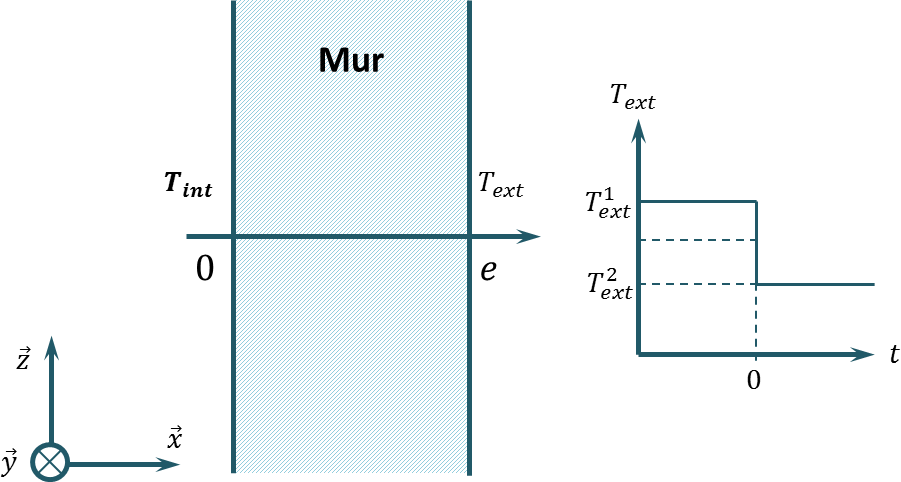
\includegraphics[width=\linewidth]{images/figure_01}
\end{center}




\begin{obj}
L'objectif est de déterminer l'évolution du flux thermique dans le mur au cours du temps. Pour cela, on s'appuiera sur la résolution d'une équation différentielle en utilisant un schéma explicite puis implicite.
\end{obj}
\fi
\subsection*{Équation gouvernant la température}
\ifprof
\else
En l'absence de source d'énergie, l'équation régissant le transport de la chaleur s'exprime ainsi :
\begin{equation}
\mathbf{\rho c_p \dfrac{\partial T(x,y,z,t)}{\partial t} =  \lambda  \Delta T(x,y,z,t)}
\end{equation}
On rappelle la définition du Laplacien d'une fonction suffisamment régulière 
$\Delta f =\frac{\partial^2 f}{\partial x^2}+\frac{\partial^2 f}{\partial y^2}
+\frac{\partial^2 f}{\partial z^2}$.
\fi

\subparagraph{}\textit{En utilisant les hypothèses dimensionnelles, donner l'équation de la chaleur simplifiée. }
\ifprof
\begin{corrige}
$$ 
\rho c_p \dfrac{\partial T(x,t)}{\partial t} =  \lambda  \dfrac{\partial^2 T(x,t)}{\partial x^2}
$$
\end{corrige}
\else
\fi

\subsection*{Conditions aux limites}
\ifprof
\else
On envisage  plusieurs types de conditions aux limites :
\begin{itemize}
\item \textbf{cas 1 : } la température est imposée aux limites du système;
\item \textbf{cas 2 : } la paroi extérieure est isolée par un matériau de très faible conductivité. 
\end{itemize}
\fi

\subparagraph{}\textit{Traduire chacune de ces conditions aux limites sur la fonction $T(x,t)$ et/ou sa dérivée.} 
\ifprof
\begin{corrige} ~\\
\begin{itemize}
\item \textbf{cas 1 : } $T(0,t)=T_{\text{int}}$ et $T(e,t)=T_{\text{ext}}$;
\item \textbf{cas 2 : } $T(0,t)=T_{\text{int}}$ et $ \dfrac{\partial T}{\partial t} (e,t)=0$.
\end{itemize}
\end{corrige}

\else
\fi

\vspace{.5cm}

\textbf{Dans la suite, seul le premier cas sera étudié.}

\subparagraph{}\textit{Résoudre l'équation de la chaleur simplifiée \textbf{en régime permanent} dans les conditions suivantes : 
\begin{itemize}
\item \textbf{conditions 1 : } pour un instant particulier négatif $t_1<0$;
\item \textbf{conditions 2 : } pour un instant particulier positif  $t_2>0$, très longtemps après la variation de température extérieure quand le régime permanent est de nouveau établi dans le mur.
\end{itemize}
} 

\ifprof
\begin{corrige} ~\\
En régime permanent, l'équation différentielle devient : $\dfrac{\partial^2 T(x,t)}{\partial x^2}=0$. On a donc :
$T(x) =  k_1 x + k_2 $. Par suite : $T(0)=T_{\text{int}}=k_2$ et $T(e)=T_{\text{ext}} = k_1 e + k_2 $. On a donc : 
$ k_1 =\dfrac{T_{\text{ext}} -T_{\text{int}}}{e} $. Au final : $T(x) =  \dfrac{T_{\text{ext}} -T_{\text{int}}}{e} x + T_{\text{int}} $.


\begin{itemize}
\item \textbf{conditions 1 : } lorsque $t_1 <0$,  $T_{\text{int}}=20^{\text{o}} \text{C}$ et $T_{\text{ext,1}}=10^{\text{o}} \text{C}$. En conséquences, $T(x) =  \dfrac{T_{\text{ext,1}} -T_{\text{int}}}{e} x + T_{\text{int}} $.
\item \textbf{conditions 2 : }  lorsque $t_2 >0$,  $T_{\text{int}}=20^{\text{o}} \text{C}$ et $T_{\text{ext,2}}=-10^{\text{o}} \text{C}$. En conséquences, $T(x) =  \dfrac{T_{\text{ext,2}} -T_{\text{int}}}{e} x + T_{\text{int}} $.
\end{itemize}
\end{corrige}
\else
\fi


\subparagraph{}\textit{Quelle est la nature des profils $T(x)$ obtenus (en régime permanent) à ces deux instants ? Tracer à la main les deux profils sur un même graphique sur la copie.}

\section*{Résolution numérique : méthode des différences finies}

\ifprof
\else
On cherche à résoudre numériquement l'équation aux dérivées partielles : 
\begin{equation}
\mathbf{\alpha \dfrac{\partial T(x,t)}{\partial t} = \dfrac{\partial^2 T(x,t)}{\partial x^2}} \quad \text{avec }\alpha \text{ constante.}
\end{equation}
Les conditions aux limites sont les suivantes :
\begin{itemize}
\item $T(0,t)=T_{\text{int}}$ pour $t>0$;
\item $T(e,t)=T_{\text{ext,2}}$ pour $t>0$;
\item $T(x,0)=ax + b$ pour $x\in[0,e]$.
\end{itemize}
\fi

\subparagraph{}\textit{Quelle est l'expression de $\alpha$ en fonction des paramètres physiques du mur ?}
\ifprof
\begin{corrige}
On a $\alpha =\dfrac{\rho c_p}{\lambda}$.

\end{corrige}

\else
\fi

\subparagraph{\label{q_tini}}\textit{Exprimer $a$ et $b$ en fonction de $T_{\text{int}}$,$T_{\text{ext,1}}$ et $e$.}
\ifprof
\begin{corrige}
On a, pour t<0, $T(0,0)= b = T_{\text{int}}$ et  $T(e,0)= ae+ T_{\text{int}}= T_{\text{ext,1}}$. On a donc : $a= \dfrac{T_{\text{ext,1}}- T_{\text{int}}}{e}$. Au final :
$$T(x,0)=\dfrac{T_{\text{ext,1}}- T_{\text{int}}}{e} x + T_{\text{int}} \quad \text{pour } x\in[0,e].$$
\end{corrige}
\else
\fi
\ifprof
\else
\vspace{.5cm}

La partie suivante permettra de déterminer une solution de l'équation aux dérivées partielles en utilisant la méthode des différences finies.

\fi
\subsection*{Discrétisation dans l'espace et dans le temps}
\ifprof
\else


On divise l'intervalle $[0,e]$, représentant l'épaisseur du mur, en $N+2$ points, numérotés de 0 à $N+1$, régulièrement espacés de $\Delta x$. Cette division est appelée << discrétisation >>. La distance $\Delta x$ est appelée le << pas d’espace >>. A l'intérieur du mur (frontières intérieure et extérieure exclues) se trouvent donc $N$ points. On cherche à obtenir la température en ces points particuliers à chaque instant. 



\begin{center}
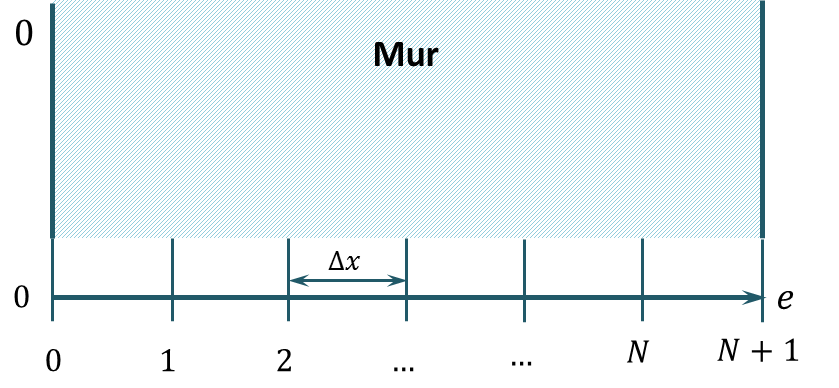
\includegraphics[width=\linewidth]{images/figure_02}
\end{center}

\fi

\subparagraph{\label{q_xini}}\textit{Donner l'expression de $\Delta x$ en fonction de $N$ et de l'épaisseur du mur $e$.}
\ifprof
\begin{corrige}
On a : $\Delta x = \dfrac{e}{N+1}$.
\end{corrige}
\else
\fi


\subparagraph{\label{q_xini2}}\textit{Donner l'abscisse $x_i$ du i\ieme point 
en fonction de $i$ et $\Delta x$, sachant que $x_0=0$ et  $x_{N+1} = e$.}
\ifprof
\begin{corrige}
On a : $x_i = i \Delta x$.
\end{corrige}
\else
\fi
\ifprof
\else
\vspace{.5cm}

Le temps est discrétisé en \textit{\text{Itmax}} intervalles de durée $\Delta t$ et on ne s'intéresse 
au profil de température qu'aux instants particuliers $t_k = k \cdot \Delta t$. 
L'intervalle élémentaire de temps $\Delta t$ est appelé le << pas de temps >>.

\noindent
Deux méthodes de résolutions sont proposées : 
\begin{itemize}
\item méthode utilisant un schéma explicite;
\item méthode utilisant un schéma implicite.
\end{itemize}
\fi

\subsection*{Méthode utilisant un schéma explicite}
\ifprof
\else
\begin{obj}
Déterminer le schéma explicite permettant la résolution de l'équation de la chaleur.
\end{obj}

On donne le développement limité à l'ordre 3 de $T(x+\Delta x,t)$ et $T(x-\Delta x,t)$ :

$
T(x+\Delta x,t)=T(x,t)+\dfrac{\partial T(x,t)}{\partial x}\Delta x  
+ \dfrac{1}{2}\dfrac{\partial^2 T(x,t)}{\partial x^2} \;\left( \Delta x\right)^2 
+ \dfrac{1}{6}\dfrac{\partial^3 T(x,t)}{\partial x^3} \;\left( \Delta x\right)^3 
+ o\left( \Delta x^3\right)
$

$
T(x-\Delta x,t)=T(x,t)-\dfrac{\partial T(x,t)}{\partial x}\Delta x 
+ \dfrac{1}{2}\dfrac{\partial^2 T(x,t)}{\partial x^2} \;\left( \Delta x\right)^2 
- \dfrac{1}{6}\dfrac{\partial^3 T(x,t)}{\partial x^3}\;\left( \Delta x\right)^3 
+ o\left( \Delta x^3\right)
$
\fi

\subparagraph{}\textit{En déduire une expression approchée à l'ordre 1 de
 $\left[\dfrac{\partial^2 T(x,t)}{\partial x^2}\right]_{x,t}$ (dérivée partielle spatiale seconde de 
 $T$ évaluée au point $x$ à l'instant $t$) en fonction de $T(x+\Delta x,t)$, $T(x-\Delta x,t)$ et 
$T(x,t)$ et $\Delta x$.}
\ifprof
\begin{corrige}
On additionne les deux lignes, on a directement :
$$
T(x+\Delta x,t)+T(x-\Delta x,t)=2T(x,t)
+ \dfrac{\partial^2 T(x,t)}{\partial x^2}(\Delta x)^2
+o((\Delta x)^3)$$
puis on isole : 
$$
\dfrac{\partial^2 T(x,t)}{\partial x^2} 
=
\dfrac{T(x+\Delta x,t)-2T(x,t) + T(x-\Delta x,t)}{\Delta x^2 }+ o\left(\Delta x\right)
$$
\end{corrige}

\else
\fi

\vspace{.5cm}

On note $T_i^k$ la température $T\left(x_i,t_k\right)$, évaluée au point d'abscisse $x_i$ à
 l'instant $t_k$. De même, on note $T_{i+1}^k=T\left(x_i + \Delta x,t_k \right)$ et 
$T_{i-1}^k=T\left(x_i - \Delta x,t_k \right)$.

\subparagraph{}\textit{Déduire de la question précédente que  
$\left[\dfrac{\partial^2 T(x,t)}{\partial x^2}\right]_{x_i,t_k} =
\dfrac{T_{i+1}^k-2T_{i}^k + T_{i-1}^k}{\Delta x^2 } $ (dérivée partielle seconde de 
$T$ évaluée en $x_i$ à l'instant $t_k$).}
\ifprof
\begin{corrige}
$$
\left[\dfrac{\partial^2 T(x,t)}{\partial x^2}\right]_{x_i,t_k} 
=
\dfrac{T_{i+1}^k-2T_{i}^k + T_{i-1}^k}{\Delta x^2 }
$$
\end{corrige}
\else
\fi
\ifprof
\else
\vspace{0.5cm}
La dérivée partielle temporelle de l'équation différentielle est maintenant approchée grâce à un
développement limité.

En utilisant le même raisonnement en réalisant un développement limité de la fonction 
$t\mapsto T(x,t)$ à l'ordre $1$, on obtiendrait l'équation suivante valable en chaque point
 d'abscisse $x_i$ et à chaque instant $t_k$ : 
$$
\left[\dfrac{\partial T(x,t)}{\partial t}\right]_{x_i,t_k} 
=
\dfrac{T_{i}^{k+1}- T_{i}^k}{\Delta t }.
$$
\fi



\subparagraph{}\textit{En utilisant les questions précédentes, montrer que 
l'équation différentielle peut se mettre sous la forme : 
$$
T_{i}^{k+1} = r T_{i-1}^{k} + \left( 1-2r \right) T_i^k + r T_{i+1}^k.
$$ 
}
$r$ sera explicité en fonction de $\Delta x$, $\Delta t$ et $\alpha$.
\ifprof
\begin{corrige}
$r=\dfrac{\Delta t}{\alpha \Delta x^2}$
\end{corrige}
\else
\fi

\ifprof
\else
\vspace{.5cm}

Dans toute la suite on considère que l'on a défini $r$ et que l'on peut l'utiliser directement. 
\vspace{.5cm}

L'équation précédente est appelée schéma numérique explicite. Si on connaît la température en tous les points $x_1$, $x_2$, ..., $x_N$ à  l'instant $t_k$ on peut calculer grâce à elle la température en tous les points à l'instant $t_{k+1}$.
\fi

\subparagraph{}\textit{L'équation est-elle valable dans tout le domaine, c'est-à-dire pour toute valeur de $i$, $0\leq i\leq N+1$ ? Que valent $T_0^k$ et $T_{N+1}^k$ ?}
\ifprof

\begin{corrige}
Oui...

On a : $T_0^k = 20^o C$ et $T^k_{N+1}=-10^o C$.  
\end{corrige}
\else
\fi


\subparagraph{}\textit{Montrer que pour tout instant $k$, le problème peut se mettre sous la forme matricielle suivante : }
$$
T^{k+1} = M \cdot T^k + rV \quad \text{avec} \quad T^k =
 \begin{pmatrix} T_1^k \\  T_2 ^k \\ ... \\  T_{N-1}^{k} \\ T_{N}^{k}  \end{pmatrix}
$$
\textit{avec M une matrice carrée $N\times N$, $V$ un vecteur de taille $N$ que l'on explicitera.}
\ifprof
\begin{corrige}
On a, pour $i\in \left]0;N+1 \right[$ :
$$
\begin{array}{ll}
i & T_{i}^{k+1} = r T_{i-1}^{k} + \left( 1-2r \right) T_i^k + r T_{i+1}^k \\
\hline 
\hline 
\\
%T_{0}^{k+1} = r T_{0-1}^{k} + \left( 1-2r \right) T_i^k + r T_{0+1}^k \\
i=1 & T_{1}^{k+1} = r T_{0}^{k} + \left( 1-2r \right) T_1^k + r T_{2}^k \\
i=2 & T_{2}^{k+1} = r T_{1}^{k} + \left( 1-2r \right) T_2^k + r T_{3}^k \\
i=3 & T_{3}^{k+1} = r T_{2}^{k} + \left( 1-2r \right) T_3^k + r T_{4}^k \\
&\\
i=N -1& T_{N -1}^{k+1} = r T_{N -2}^{k} + \left( 1-2r \right) T_{N -1}^k + r T_{N}^k \\
i=N & T_{N}^{k+1} = r T_{N-1}^{k} + \left( 1-2r \right) T_N^k + r T_{N+1}^k \\
\end{array}
$$ 

On a donc : 
$$
T^{k+1} = M \cdot T^k + rV
$$
avec :
$$
M = 
\begin{pmatrix}
1-2r & r     & 0 & 0 & 0 &  \ldots & 0 \\
r     & 1-2r & r & 0 & 0  & \ldots &  0 \\
0    & r & 1-2r & r & 0   & \ldots&  0 \\
\vdots & \vdots & \vdots & \vdots & \vdots & \ldots & \ldots \\
0& 0& 0& 0& 0& r & 1-2r\\
\end{pmatrix}
\quad \text{et} \quad 
V = \begin{pmatrix}
T_0^k = T_{\text{int}} \\
0 \\
\vdots \\
0 \\
T_N^k = T_{\text{ext,2}} \\
\end{pmatrix}.
$$
\end{corrige}
\else
\fi
%\subparagraph{}
%\textit{Donner toutes les composantes de $T^0$.}
%\begin{corrige}
%\end{corrige}
%\ifprof
%\else
%\fi
\ifprof
\else
\vspace{.5cm}
Ainsi, à chaque pas de temps $k$, on calculera un vecteur $T^k$ contenant la température à chaque abscisse $i$ du mur.

\begin{center}
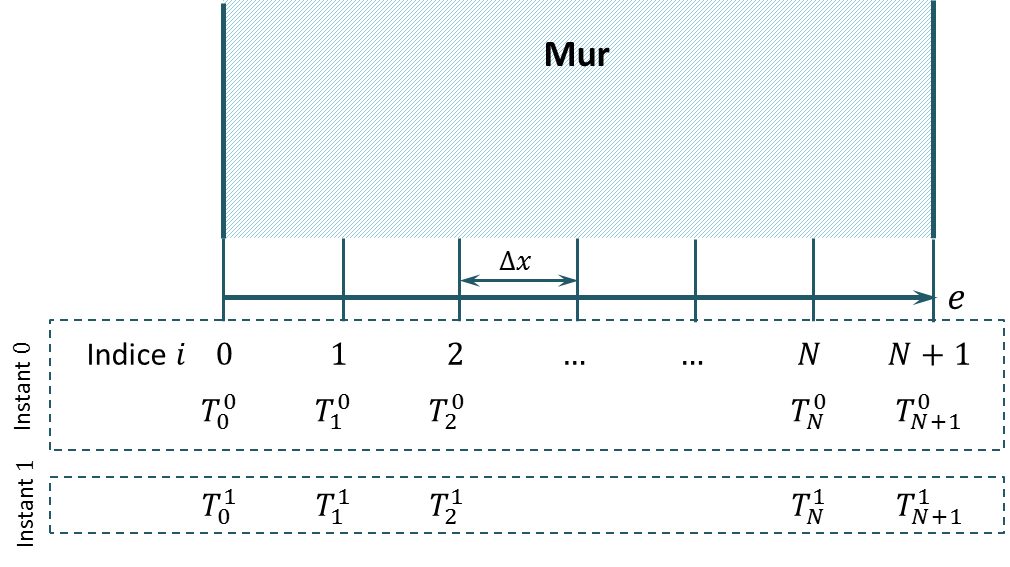
\includegraphics[width=\linewidth]{images/figure_03}
\end{center}
\fi

\subparagraph{}
\textit{Expliciter succinctement comment déterminer la température dans le mur à chaque instant.}
\ifprof
\begin{corrige}
\`A l'instant $t=0$, le flux de température dans le mur est connu. La température extérieure passe alors à $-10^o C$. On utilise alors l'équation de récurrence.

(Lors du codage de la méthode explicite, il faut faire attention à la divergence du schéma. Pour cela, il faut prendre des intervalles de temps << petits >>.)
\end{corrige}
\else
\fi
%
%\ifprof
%\else
%\vspace{.5cm}
%
%\noindent
%Une annexe est fournie en fin de sujet vous rappelant quelques fonction de la bibliothèque \textbf{Numpy}.
%\fi

\subparagraph{}
\textit{On donne \texttt{ T0} le vecteur température à l'instant $k=0$. 
Écrire la fonction \texttt{euler\_explicite(M,T0,V,k)} retournant le vecteur de température 
$T^k$ à l'instant $k$. Cette fonction sera définie de manière \textbf{récursive}.}\\

\ifprof
\begin{corrige}
~\\
\begin{python}
def euler_explicite(M,T_0,r,V,k):
    if k==1:
        return np.dot(M,T_0)+r*V
    else:
        T=euler_explicite(M,T_0,r,V,k-1)
        return np.dot(M,T)+r*V
        
\end{python}
\end{corrige}
\else
\fi




\subsection*{Méthode utilisant un schéma implicite}
\ifprof
\else
\begin{obj}
Déterminer une méthode permettant de résoudre l'équation de la chaleur à partir du 
schéma implicite donné.
\end{obj}

En utilisant un schéma d'Euler implicite, on montre que l'équation 
$\alpha \dfrac{\partial T(x,t)}{\partial t} = \dfrac{\partial^2 T(x,t)}{\partial x^2}$
 peut se mettre sous la forme suivante : 
$$
T_i^k = -rT_{i-1}^{k+1} + \left( 1+2r\right) T_{i}^{k+1}-rT_{i+1}^{k+1}.
$$

La température à l'instant $t_k$ est exprimée en fonction de la température à l'instant 
ultérieur $t_{k+1}$.
Le système d'équation peut être écrit sous la forme matricielle : 
\begin{equation} \label{eq_implicite}
\mathbf{M T^{k+1} = T^k + rV}
\end{equation}
avec : 

$$
M = 
\begin{pmatrix}
1+2r & -r     & 0 & 0 & 0 &  \ldots & 0 \\
-r     & 1+2r & -r & 0 & 0  & \ldots &  0 \\
0    & -r & 1+2r & -r & 0   & \ldots&  0 \\
\vdots & \vdots & \vdots & \vdots & \vdots & \ldots & \ldots \\
0& 0& 0& 0& 0& -r & 1+2r\\
\end{pmatrix}
$$

$$ 
V = \begin{pmatrix}
T_{\text{int}} \\
0 \\
\vdots \\
0 \\
T_{\text{ext}} \\
\end{pmatrix}
\quad
T^k = \begin{pmatrix}
T_1^k \\
T_2^k  \\
\vdots \\
T_{N-1}^k  \\
T_N^k \\
\end{pmatrix}.
$$

\fi


\subparagraph{}
\textit{Pour obtenir $T^{k+1}$ en fonction de $T^{k}$, il est nécessaire d'inverser le 
système matriciel à chaque pas de temps.
Donner le nom d'un algorithme permettant de faire cela et donner sa complexité.}

\ifprof
\begin{corrige}
On peut utiliser l'algorithme du pivot de Gauss. Sa complexité est en $\mathcal{O}(n^3)$.
\end{corrige}
\else
\fi

\ifprof
\else

\begin{obj}
La matrice $M$ étant particulière (tridiagonale) , nous allons utiliser un algorithme plus 
performant pour résoudre ce système matriciel tridiagonal : l'algorithme de Thomas.
 Le système que l'on cherche à résoudre est le suivant : 
$$
M U = D 
$$
$M$ est une matrice tridiagonale de dimension $N\times N$, c'est à dire que tous les éléments 
sont nuls sauf les diagonales principales, supérieures et inférieures. 
\end{obj}

On a donc : 
$$
M = 
\begin{pmatrix}
b_0 & c_0 &  &  &  &  & \\
a_1 & b_1 & c_1 & &0 & &\\
      & a_2 & b_2 & c_2 & & & \\
& & \ddots & \ddots & \ddots & \\
& 0& & a_{N-2} & b_{N-2} & c_{N-2}\\
& & & & a_{N-1} & b_{N-1}\\
\end{pmatrix}
$$

$$
U = \begin{pmatrix}
u_0 \\
\vdots \\
\vdots \\
\vdots  \\
u_{N-1} \\
\end{pmatrix}
\quad 
D = \begin{pmatrix}
d_0 \\
\vdots \\
\vdots \\
\vdots  \\
d_{N-1} \\
\end{pmatrix}.
$$

Dans cet algorithme, on calcule les coefficients suivants : 
$
c'_0 = \dfrac{c_0}{b_0} \quad c'_i = \dfrac{c_i}{b_i - a_i c'_{i-1}}  \quad \text{pour} \quad i=1,2,\ldots, N-2$

et $
d'_0 = \dfrac{d_0}{b_0} \quad d'_i = \dfrac{d_i-a_i d'_{i-1}}{b_i - a_i c'_{i-1}}  \quad \text{pour} \quad i=1,2,\ldots, N-1.
$

Les inconnues $u_0, u_1, \ldots, u_{N-1}$ sont alors obtenues par les formules :
$
u_{N-1} = d'_{N-1} \quad u_i = d'_i -c'_i u_{i+1} \quad  \text{pour} \quad i=N-2, N-3, \ldots, 1, 0.
$

\fi

\subparagraph{}
\textit{En utilisant l'algorithme de Thomas, écrire une fonction \texttt{CalcTkp1(M,D)} 
qui retourne le vecteur $U$, solution du système matriciel, à partir de la matrice 
$M$ et du vecteur $D$.}\\

On pourra commencer par créer  des vecteurs contenant des zéros :
 A, B, C, Cp ,Dp (pour C' et D') et U.\\
 Puis on pourra  définir A, B et C à partir de la matrice $M$ et ensuite calculer Cp et Dp puis U.

\ifprof
\begin{corrige}
~\\
Proposition de corrigé qui ne correspond pas exactement aux préconisations de l'énoncé :

\begin{python}
def CalcTkp1(M,d):
    N=d.shape[0]
    c=[M[0,1]/M[0,0]]
    d_prime=[d[0,0]/M[0,0]]
    u=np.zeros((N,1))
    for i in range(1,N-1):
        c.append(M[i,i+1]/(M[i,i]-M[i,i-1]*c[i-1]))
        d_prime.append((d[i,0]-M[i,i-1]*d_prime[-1])/(M[i,i]-M[i,i-1]*c[i-1]))
    d_prime.append((d[N-1,0]-M[N-1,N-2]*d_prime[-1])/(M[N-1,N-1]-M[N-1,N-2]*c[-1]))
    u[N-1,0]=d_prime[-1]
    for j in range(2,N):
        u[N-j,0]=d_prime[N-j]-c[N-j]*u[N-j+1,0]
    return u
\end{python}
\end{corrige}
\else
\fi

\subparagraph{}
\textit{Donner la complexité de l'algorithme et comparer à celui de la question 16. 
On prendra en compte uniquement les tests, les affectations (même de tableaux)
 et les opérations élémentaires (+, -, *, /) qui compte chacune pour << un >>.}\\

\ifprof
\begin{corrige}
La complexité de l'algorithme est linéaire (à comparer à une complexité cubique pour l'algorithme de Gauss).
\end{corrige}
\else
\fi


\section*{Résolution de l'équation différentielle implicite}
\ifprof
\else
L'objectif est de calculer la température en chaque point au cours du temps. Parmi les variables
d'entrée se trouvera un vecteur $T_0$ de dimension $N$, défini en dehors de la fonction,
 contenant les valeurs de la température aux points de discrétisation à l'instant initial. 
 Au sein de la fonction, un algorithme calculera itérativement la température avec un 
 nombre maximal d'itérations \text{Itmax}. En sortie de la fonction, on récupérera le nombre 
 d'itérations réellement effectuées, \texttt{nbIter} et une matrice \texttt{T\_tous\_k}, de
  dimensions $N\times \text{\text{Itmax}}$.  Chaque colonne de cette matrice contient le vecteur $T^k$
   dont les éléments sont les valeurs de la température aux $N$ points $x_1$, ..., $x_N$, 
 points à l'intérieur du mur à l'instant $k$ :
$$
T^k = \begin{pmatrix} T_1^k \\  T_2 ^k \\ ... \\  T_{N-1}^{k} \\ T_{N}^{k}  \end{pmatrix}
$$

$$
T\_\text{tous}\_k = 
\begin{pmatrix} 
T_1^1   & T_1^2  & \cdots & T_1^{\text{Itmax}-1} & T_{1}^{\text{Itmax}} \vspace{0.3cm} \\
T_2^1   & T_2^2  & \cdots & T_2^{\text{Itmax}-1} & T_2^{\text{Itmax} }  \vspace{0.15cm}\\
\vdots & \vdots & \cdots & \vdots & \vdots \vspace{0.15cm}\\
T_{N-1}^1   & T_{N-1}^2  & \cdots & T_{N-1}^{\text{Itmax}-1} & T_{N-1}^{\text{Itmax}} \vspace{0.3cm} \\
T_{N}^1   & T_{N}^2  & \cdots & T_{N}^{\text{Itmax}-1} & T_{N}^{\text{Itmax}}  \\
 \end{pmatrix}.
$$


On souhaite arrêter le calcul lorsque la température ne varie presque plus dans le temps. 
Dans ce but, on évaluera la norme  de $T^k - T^{k-1}$ à chaque itération. 
\begin{defi}
On définit la norme d'un vecteur $v$ par : 
$$
||v|| = \sqrt{\sum\limits_{i=1}^{N}v_i^2} \quad \text{avec} \quad v=
\begin{pmatrix} v_1 \\ v_2 \\ \vdots \\ \vdots \\ v_n \end{pmatrix}.
$$
\end{defi}

\fi

\subparagraph{}
\textit{Écrire une fonction \texttt{calc\_norme} qui calcule la norme d'un vecteur. }
\ifprof
\begin{corrige}
 ~\\
\begin{python}
def calc_norme(v):
    res = 0
    for i in range(len(v)):
        res = res+v[i]**2
    return math.sqrt(res)        
\end{python}
\end{corrige}
\else
\fi

%\subparagraph{\label{q_solve}}
%\textit{Écrire \textbf{l'en-tête} de la fonction \texttt{schema\_implicite} permettant de calculer la température en chaque point au cours du temps. Vous préciserez clairement les paramètres d'entrée et de sortie.}
\subparagraph{\label{q_solve}}
\textit{Écrire la fonction \texttt{solution(M,T,V)}, d'arguments une matrice $M$
 tridiagonale et deux vecteurs $T$ et $V$ et retournant le vecteur $U$ tels que $MU=T+rV$.}
 On utilisera la fonction \texttt{CalcTkp1}.
\ifprof   
\begin{corrige}
\begin{python}
def solution(M,T,V) :
    """
    Entrées : 
        * M, np.array (N+1 x N+1) : matrice à inverser
        * T, np.array (N+1 x 1) : température à chaque abscisse du mur à l'instant k
        * V, np.array (N+1 x 1) : température *imposée* à chaque abscisse du mur à l'instant final
    Sortie : 
        * TT, np.array (N+1 x 1) : température à chaque abscisse du mur à l'instant k+1
    """
    # On considère que r a été définie auparavant comme variable globale.
    D = T+r*V
    return CalcTkp1(M,D)
\end{python}
\end{corrige}
\else
\fi

\subparagraph{}
\textit{Affecter la valeur 2000 à  \texttt{ \text{Itmax}}. Créer la matrice  \texttt{T\_tous\_k}  de dimensions $N\times \text{Itmax}$ en la remplissant de zéros.}
\ifprof
\begin{corrige}
~\\
\begin{python}
\text{Itmax} = 2000
T_tous_k = np.zeros([N,\text{Itmax}])
\end{python}
\end{corrige}
\else
\fi


\subparagraph{}
\textit{D'après les questions précédentes la température $T$ dans le mur vérifie la condition
 initiale  $T(x,0)=ax+b$ où 
 $a=\dfrac{T_{\text{ext},1}-T_{\text{int}}}{e}$  et  $b=T_{\text{int}}$.\\
Écrire la fonction \texttt{T0(Tint,Text,N) } d'arguments la température intérieure $T_{\text{int}}$, 
la température extérieure $T_{\text{ext}}$ et l'entier $N$ et retournant le vecteur $T^0$, de taille $N$,
contenant les températures en chaque point du mur lorsque $t=0$. }
%\textit{En utilisant les résultats des questions \ref{q_tini}, \ref{q_xini} et \ref{q_xini2}, 
%écrire la fonction T0(Tint,Text,N) d'arguments la température intérieure $Tint$, 
%la température extérieure $Text$ et l'entier $N$ et retournant le vecteur $T^0$, de taille $N$,
%contenant les températures en chaque point du mur lorsque $t\leq 0$. }
\ifprof
\begin{corrige} 
On a : $T(x_i,k=0)=\dfrac{T_{\text{ext},1}-T_{\text{int}}}{e}x_i + T_{\text{int}} = \dfrac{T_{\text{ext},1}-T_{\text{int}}}{e}\cdot i \cdot \dfrac{e}{N+1} + T_{\text{int}} =  \dfrac{T_{\text{ext},1}-T_{\text{int}}}{N+1}\cdot i  + T_{\text{int}}$.
~\\
\begin{python}
def T0(Ti,Tf,N):
    tt =  np.zeros((N,1))
    for i in range(N):
        tt[i] = ((Tf-Ti)/(N-1))*i+Ti #si il y a N points on a divisé l'intervalle en N-1
    return tt
\end{python}
\end{corrige}
\else
\fi



\subparagraph{}
\textit{Écrire la suite d'instructions qui affecte à la première colonne de \texttt{T\_tous\_k} 
 le vecteur des valeurs initiales $T^0$. }
 On utilisera la fonction \texttt{T0}. 
\ifprof
\begin{corrige}~\\

\begin{python}
t0 = T0(Tint,Text1,N)
for i in range(N):
    T_tous_k[i][0] = t0[i]
\end{python}
\end{corrige}
\else
\fi



\subparagraph{}
\textit{Écrire les instructions permettant de définir $M$ et le vecteur $V$ qui interviennent dans l'équation \ref{eq_implicite}. }
\ifprof
\begin{corrige} ~\\
\begin{python}
M = np.zeros((N,N))
M[0][0]=1+2*r
M[0][1]=-r

M[N-1][N-1]=1+2*r
M[N-1][N-2]=-r
for i in range(1,N-1):
    M[i][i]=1+2*r
    M[i][i+1]=-r
    M[i][i-1]=-r

V = np.zeros((N,1))
V[0][0]=Tint
V[N-1][0]=Text2
\end{python}
\end{corrige}

\else
\fi


\subparagraph{}
\textit{Donner la suite d'instructions permettant de calculer le profil de la température à 
l'instant $k=1$ ($t=\Delta t$). C'est à dire le vecteur $T^1$ .}
On utilisera la fonction  \texttt{solution}.%On utilisera la fonction  \texttt{schema\_implicite}.
\ifprof

\begin{corrige}
%Tk =  calcTkp1(M,T_tous_k[:][0]) + r*CalcTkp1(M,V) 
\begin{python}
T1=solution(M,T0,V)
\end{python}
\end{corrige}
\else
\fi


\subparagraph{}
\textit{Écrire la fonction \texttt{euler\_implicite(M,T0,V)} d'argument une matrice $M$ et 
deux vecteurs $T0$ et $V$ et renvoyant la matrice \texttt{ T\_tous\_k}.\\
Cette boucle sera interrompue lorsque la norme  du vecteur $T^k-T^{k-1}$ deviendra inférieure à $10^{-2}$ ou lorsque le nombre d'itérations atteindra la valeur \text{Itmax} (prévoir deux cas). Utiliser pour cela les fonctions \texttt{calc\_norme} et \texttt{solution} définies précédemment.}
%\textit{Élaborer une boucle permettant de calculer itérativement le profil de température aux instants $t_k = k \Delta t$ avec $k\geq 2$. Cette boucle sera interrompue lorsque la norme 2 du vecteur $T^k-T^{k-1}$ deviendra inférieure à $10^{-2}$ ou lorsque le nombre d'itérations atteindra la valeur \text{Itmax} (prévoir deux cas). Utiliser pour cela la fonction \texttt{calc\_norme} définie précédemment.}
\ifprof


\begin{corrige}
Bloc d'instructions à intégrer dans la fonction \texttt{euler\_implicite(M,T0,V)} :
\begin{python}
v=np.zeros((T_tous_k.shape[0],1))
for i in range(T_tous_k.shape[0]):
    v[i,0]=T_tous_k[i,1]-T_tous_k[i,0]
k=1
T=T0(Tint,Text,N)
while calc_norme(v)>10**(-2) and k!=\text{Itmax}:
    k=k+1
    T=solution(M,T,V)
    for i in range(T_tous_k.shape[0]):
        T_tous_k[i,k]=T[i,0]
        v[i,0]=T_tous_k[i,k]-T_tous_k[i,k-1]
\end{python}        
\end{corrige}
\else
\fi



%\subparagraph{}
%\textit{Écrire la fin de la fonction afin de renvoyer tous les arguments de sortie définis au
%début de la question \ref{q_solve}.}
%\ifprof
%
%\begin{corrige}
%\end{corrige}
%\else
%\fi


\section*{Analyse des résultats}
\ifprof
\else
12 heures sont nécessaires pour atteindre le régime permanent. En utilisant le schéma implicite, on souhaite afficher la courbe de température en fonction de l'abscisse du mur. Le graphe attendu est le suivant :

\begin{center}
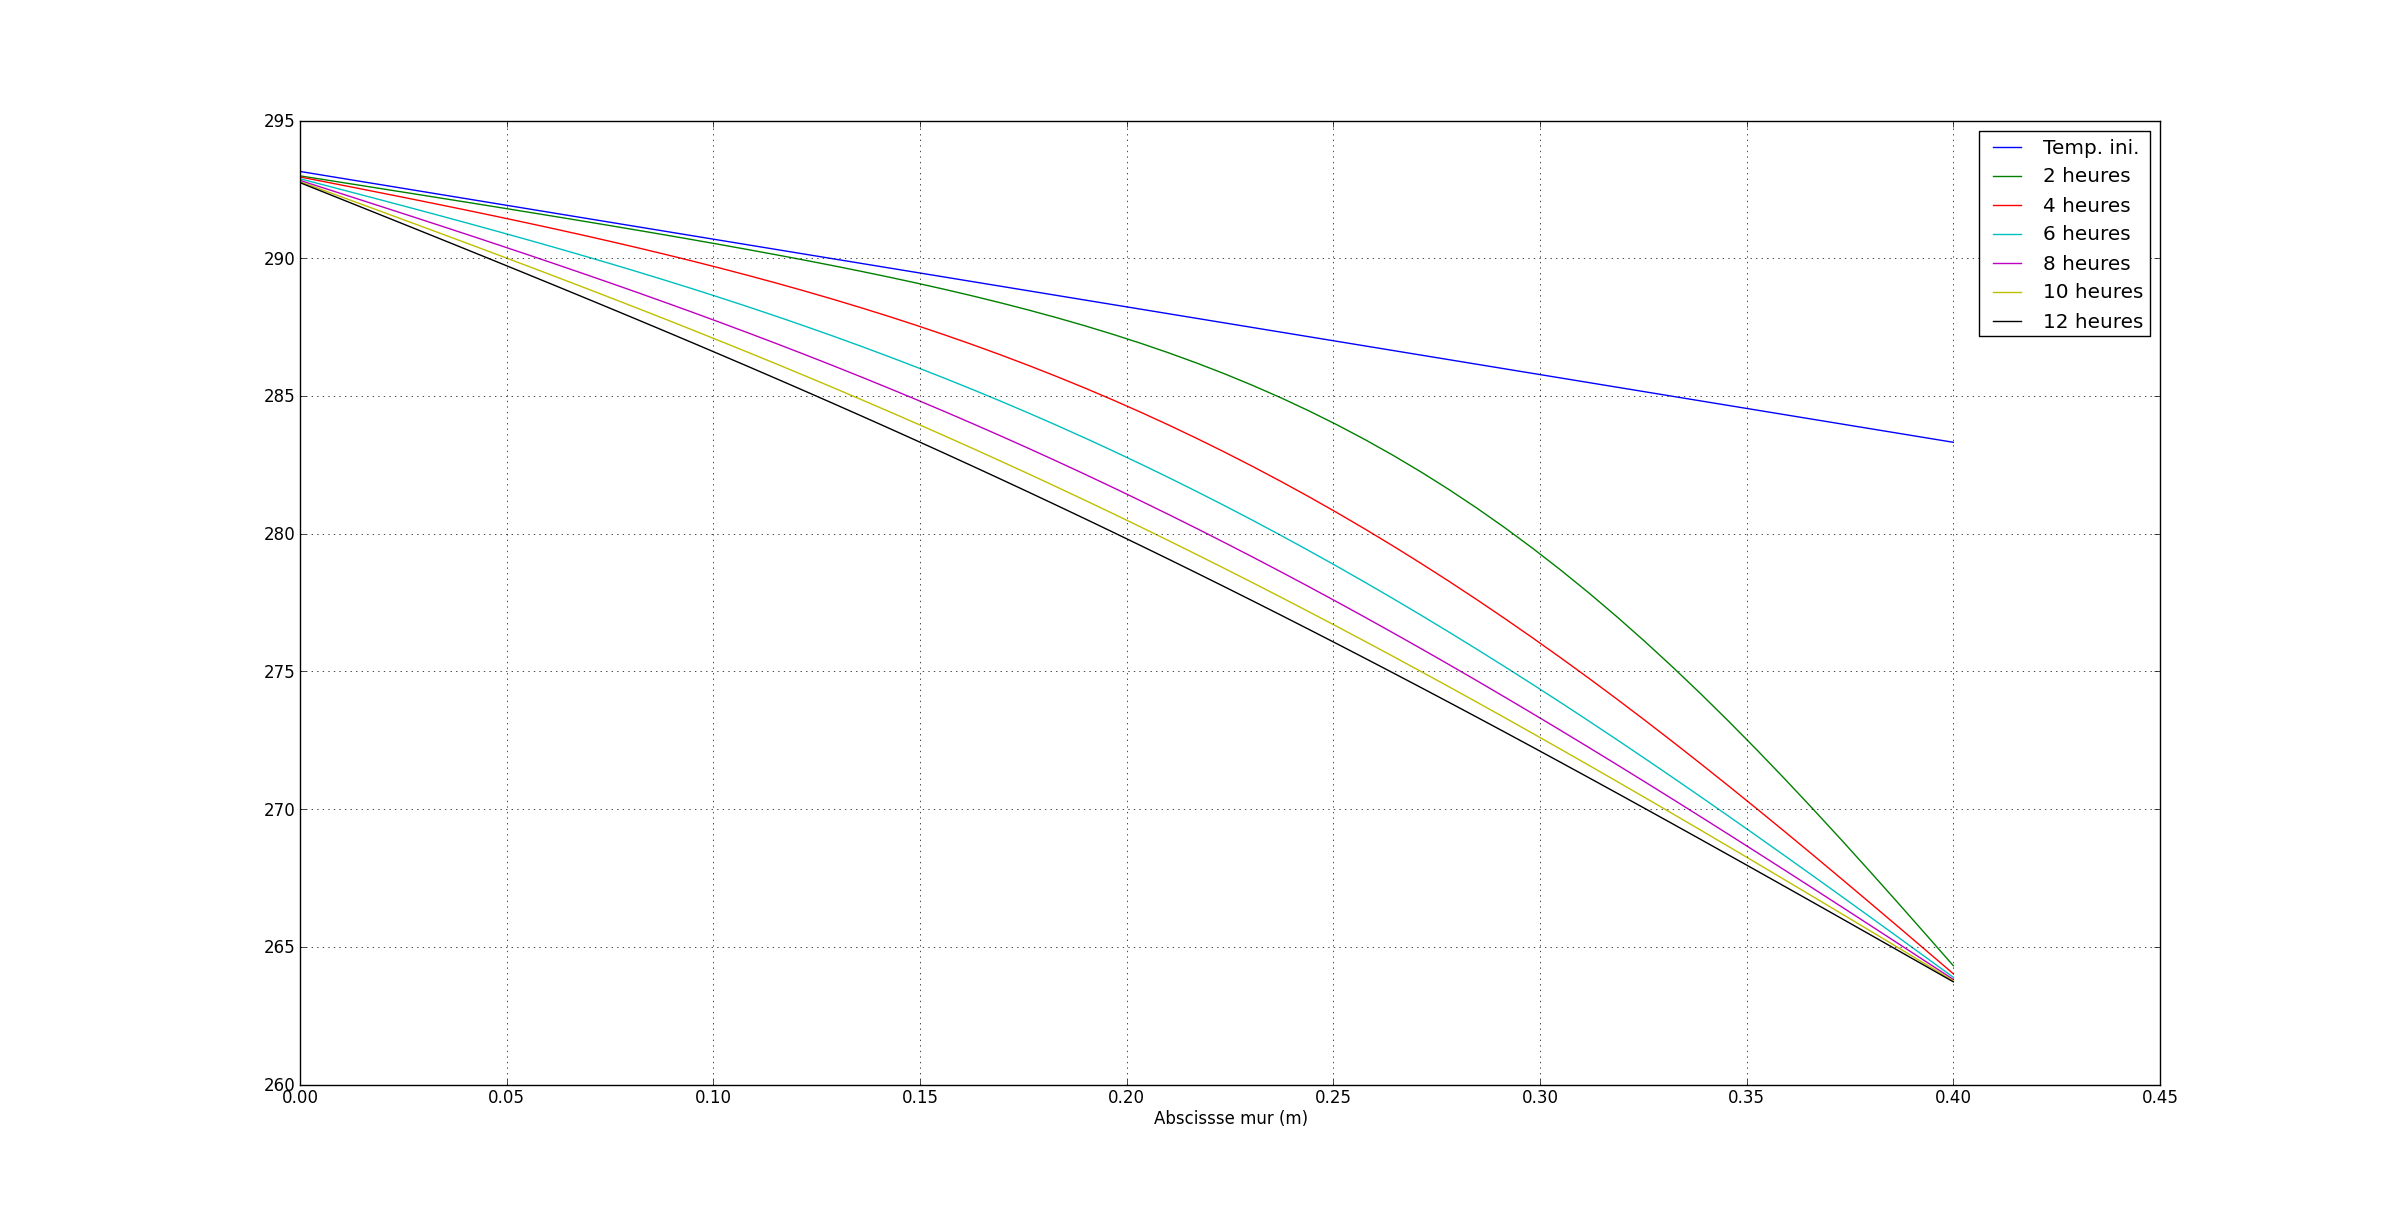
\includegraphics[width=\linewidth]{images/figure_04}
\end{center}

\fi

\subparagraph{}
\textit{Le pas de discrétisation temporel est de 30 secondes. Les résultats de la simulation sont stockés dans la matrice  \texttt{ T\_tous\_k}  définie précédemment. Écrire les instructions permettant de tracer le réseau de courbes précédentes.}
\ifprof

\begin{corrige}
~\\
\begin{python}
k=[0,240,480,720,960,1200,1440]
les_X=[i*0.4/(N+1) for i in range(N+2)]
for i in k:
    plt.plot(les_X,T_tous_k[:,i])
plt.show()
\end{python}
\end{corrige}
\else
\fi

\ifprof
\else
\vspace{.5cm}

Les résultats de la simulation sont codés dans un fichier texte codé en ASCII. L'écriture des nombres est limitée à 10 caractères (signe et virgule inclus). 
Le mur est discrétisé en 100 abscisses. Le pas de discrétisation temporel est de 30 secondes. 
\fi

\subparagraph{}
\textit{Quelle sera la taille du fichier texte généré ?}
\ifprof
\begin{corrige}
Si on considère que $\text{Itmax}=2000$, on aura donc $100 \times 2000$ valeurs. Pour l'estimation de la taille du fichier on fait ici l'abstraction du codage des espaces et des retours à la ligne. 
La taille du fichier est donc : $100 \times 2000 \times 10 \times 1 \simeq 2\, \text{Mo}$.
\end{corrige}
\else
\fi
%
%\ifprof
%\else
%\section*{Annexe}
%\noindent
%Dans tout le problème, on suppose que la bibliothèque \textbf{Numpy} a été chargée.\\
%Tous les vecteurs et matrices intervenant seront des tableaux de numpy (array).\\
%Par exemple, on peut définir des vecteurs par :\\
% $U=array([1,2,3])$ et $V=array([1,0,1]]$.\\
%On a comme pour des listes : $U[0]=1, U[1]=2, V[1]=0$...\\
%On peut définir une matrice par $M=array([[1,1,2],[1,-1,0],[0,1,3]])$ c'est la matrice
% $M=\left(\begin{array}{ccc}1&1&2\\1&-1&0 \\ 0&1&3 \end{array} \right)$.\\
%De même , par exemple, on a $M[0,2]=2$. \\
%On peut additionner deux vecteurs : $U+V=array([2,2,4])$, multiplier par un scalaire :
%$3*U=array([2,6,9])$ .\\
%Pour effectuer le produit scalaire on fait \textbf{vdot(u,v)}.\\
%Pour effectuer le calcul de $MU$ on fait \textbf{dot(M,U)}.\\
%On peut aussi définir un vecteur de taille $N$ contenant des zéros par l'instruction 
%$A=$\textbf{zeros([N])} et une matrice de taille $i\times j$ contenant des zéros par 
%$M=$\textbf{zeros([i,j])} .
%\fi
%

\ifprof
\else
\end{multicols}
\fi
\end{document}




